% !TeX encoding = UTF-8
% !TeX program = xelatex
% !TeX spellcheck = en_US

\documentclass[degree=doctor,language=chinese,font=external,cjk-font=external]{sustechthesis}
  %%%%%%%%%%%%%%%%%%%%%%%%
  %   研究生学位论文模板
  %%%%%%%%%%%%%%%%%%%%%%%%

  % 学位 degree:
  %   master (默认) | doctor
  % 语言 language:
  %   chinese (默认)| english
  % 英文字体 font
  %   auto (默认,自动选择系统自带字体)| external (包内字体)| times | termes | 等
  %   Windows 和 macOS 系统上,无需设定。系统自带对应字体,可以删除该参数。
  %   Unix 系统推荐使用包内字体,而非TeX自带的克隆版字体,以达到和其他系统一致的字体效果。
  %   Windows 系统上可以删除该参数,使用系统内置字体。
  % 中文字体 cjk-font
  %   auto (默认,自动选择系统自带字体)| external (包内字体)| windows | mac | 等
  %   在 **非Windows** 的系统上推荐使用包内字体,而非系统字体。
  %   以达到和 Windows 系统一致的字体效果。
  %   Windows 系统自带对应字体,可以删除该参数。


% 论文基本配置,加载宏包等全局配置
% 在此文件中可以选择
% 1. 生成的PDF为无空白页的用于电子版提交的版本 或 插入空白页的以便双面打印的版本
% 2. 学位学科门类(理学、工学、医学)
% 3. 培养单位
% 4. 作者姓名、指导教师等
% 5. 修改gongshuo的值, 默认为false代表生成学术型研究生毕业设计模板, 改为true则将生成专业型研究生毕业设计模板
% !TeX root = ./sustechthesis-example.tex

% 论文基本信息配置

\thusetup{
  %******************************
  % 注意:
  %   1. 配置里面不要出现**空行**
  %   2. 不需要的配置信息可以删除
  %   3. 建议先阅读文档中所有关于选项的说明
  %******************************
  %
  % 输出格式
  %   选择打印版(print)或用于提交的电子版(electronic),前者会插入空白页以便直接双面打印
  %
  output = electronic,
  %
  % 文档类型
  %   选择开题报告(proposal)、年度考核报告(progress)或学位论文(thesis)【默认值】。
  %
  type = thesis,
  %
  % 标题
  %   可使用“\\”命令手动控制换行
  %   如果需要使用副标题,取消 subtitle 和 subtitle* 的注释即可。
  %   特别字符允许小写,例如行内公式,其他所有字词全部大写。
  %
  title  = {Robotics model and control},
  title* = {Quadrupedal Robots Motion Model and Control Strategies},
  % subtitle = {可选的副标题可选的副标题可选的副标题可选的副标题可选的副标题可选的副标题},
  % subtitle* = {optional subtitle optional subtitle optional subtitle optional subtitle optional subtitle optional subtitle},
  %
  % 学位
  %
  degree-domain = {工学}, % 【中文】学科门类:可选理学、工学、医学
  degree-domain* = {Engineering}, % 【英文】学位等级:可选Science, Engineering, Medicine
  gongshuo = false, % 是否为专业型学位。专业型学位则填 true ,学术型或其他为 false 。
  %
  % 培养单位
  %   填写所属院系的全名
  %   超长英文系名可以手动换行
  department = {量子科学与工程研究院},
  department* = {Institute of Quantum Science and Engineering},
  %
  % 学科
  %   1. 学术型学位
  %      获得一级学科授权的学科填写一级学科名称,其他填写二级学科名称
  %   2. 工程硕士
  %      工程领域名称
  %
  discipline  = {电子科学与技术},
  discipline* = {Electronic Science and Technology},
  %
  % 姓名
  %   英文用全拼,姓在前,名在后,姓和名的首字母大写,其余小写
  %
  author-id  = {12132850},
  author  = {彭道杰},
  author* = {PENG Daojie},
  %
  % 指导教师
  %   一般情况下,只写一名指导教师。
  %   填写导师姓名,后衬导师职称“教授”,“副教授”,“研究员”等
  %
  supervisor  = {Xxx},
  supervisor* = {Assistant Prof. Xxx},
  % 副指导教师
  %   一般无需启用该项,留空或者注释掉即可。
  %   如需启用限填写一名,且需要向学位办确认和备案,职称要求同指导教师。
  % associate-supervisor  = {大卫查理助理教授},
  % associate-supervisor* = {Assistant Prof. David Charlie},
  %
  % 日期
  %   使用 ISO 格式;默认为当前时间
  %   date 为第一页全中文大写日期,defense-date 为第二、三页的答辩日期。
  %   需要按 {年-月-日} 格式填写,如不显示“日”,可以随意填一个日期,但是不能为空。
  %
  date = {2023-09-20},
  defense-date = {2023-09-20},
  %
  % 密级
  %   公开, 秘密, 机密, 绝密
  %
  statesecrets={公开},
  %
  % 国内图书分类号:查询网址:https://ztflh.xhma.com/
  %   国内图书分类号可先参考知网上类似学位论文的分类号,再进行确认。
  % 国际图书分类号,查询网址:https://udcsummary.info/php/index.php?lang=chi
  %
  natclassifiedindex={XXxxx.x},
  intclassifiedindex={xx-x},
}

\thusetup{
  %
  % 数学字体
  % math-style = GB,  % GB (中文默认) | TeX (英文默认)
  math-font  = cambria,  % cambria (默认,同 Word 默认数学字体一致) | times (Times New Roman 的TeX克隆版)| xits | stix
}

% 载入所需的宏包

% 可以使用 nomencl 生成符号和缩略语说明
% \usepackage{nomencl}
% \makenomenclature

% 表格加脚注
\usepackage{threeparttable}

% 表格中支持跨行
\usepackage{multirow}

% 量和单位
\usepackage{siunitx}

% 定理类环境宏包
\usepackage{amsthm}
% 也可以使用 ntheorem
% \usepackage[amsmath,thmmarks,hyperref]{ntheorem}

%%%%%% 顺序编码制的文献引用形式
%%%%%% 参考文献编译方式二选一,不要同时开启。
%%%% 选择一:使用 BibTeX + natbib 宏包
\usepackage[sort&compress]{gbt7714}
\citestyle{super} % 全局上标数字模式
% \citestyle{numbers} % 全局行内数字模式,在写作指南2022年8月23日版本已废弃, 并决定中英文都采用上标数字格式
\bibliographystyle{sustechthesis-numeric}

%%%% 选择二:使用 BibLaTeX 宏包(兼容性不佳,不太推荐)
% \usepackage[backend=biber,style=gb7714-2015,gbalign=left]{biblatex}
% \addbibresource{ref/refs.bib} % 声明 BibLaTeX 的数据库

% 定义所有的图片文件在 figures 子目录下
\graphicspath{{figures/}}

% 数学命令
\newcommand\dif{\mathop{}\!\mathrm{d}}  % 微分符号

% hyperref 宏包在最后调用
\usepackage{hyperref}
\usepackage{ragged2e}

% 固定宽度的表格。放在 hyperref 之前的话,tabularx 里的 footnote 显示不出来。
\usepackage{tabularx}

% 跨页表格,必须在 hyperref 之后使用否则会报错。
\usepackage{longtable}

% % 源代码 minted 高亮,二选一即可。【不再推荐,会有兼容性问题:导致图表间距异常】
% %% 使用 minted 包有内置高亮颜色,需要 Python 环境编译,并安装 Pygement 包。
% \usepackage{minted}

% 源代码 listings 高亮,二选一即可。
\usepackage{listings}
%% 使用 listings 包需要自行定义高亮颜色,此处给出 Java 的例子。
\definecolor{javared}{rgb}{0.6,0,0} % for strings
\definecolor{javagreen}{rgb}{0.25,0.5,0.35} % comments
\definecolor{javapurple}{rgb}{0.5,0,0.35} % keywords
\definecolor{javadocblue}{rgb}{0.25,0.35,0.75} % javadoc

\lstset{language=Java,
  keywordstyle=\color{javapurple}\bfseries,
  stringstyle=\color{javared},
  commentstyle=\color{javagreen},
  morecomment=[s][\color{javadocblue}]{/**}{*/},
  numbers=left,
  numberstyle=\tiny\color{black},
  stepnumber=1,
  numbersep=10pt,
  tabsize=4,
  showspaces=false,
  showstringspaces=false
}

% 伪代码环境
\usepackage[ruled,linesnumbered]{algorithm2e}
% 定义伪代码的continue
\SetKw{Continue}{continue}
\SetKw{Break}{break}
% 定义算法注释
\SetKwComment{Comment}{/* }{ */}
\SetKwComment{SingleComment}{// }{}
\SetKwComment{TriComment}{$\triangleright$\ }{}

% tabular 扩展命令
\newcolumntype{R}[1]{>{\raggedleft\arraybackslash}p{#1}} % 定义R为表格左右居左,用于自定义表格列宽度
\newcolumntype{L}[1]{>{\raggedright\arraybackslash}p{#1}} % 定义L为表格左右居右,用于自定义表格列宽度
\newcolumntype{C}[1]{>{\centering\arraybackslash}p{#1}} % 定义C为表格左右居中,用于自定义表格列宽度

% tabularx 扩展命令,会对单元格内容进行单元格内自动换行
% X 默认就是两端对齐
% Y 左对齐
\newcolumntype{Y}{>{\raggedright\arraybackslash}X}
% Z 右对齐
\newcolumntype{Z}{>{\raggedleft\arraybackslash}X}
% A 居中对齐
\newcolumntype{A}{>{\centering\arraybackslash}X}

% 表格旋转
\usepackage{rotating}


\newcommand\undefcolumntype[1]{\expandafter\let\csname NC@find@#1\endcsname\relax}
\newcommand\forcenewcolumntype[1]{\undefcolumntype{#1}\newcolumntype{#1}}

% ------------------------另外自添加的外部文档引入包---------------------------
\usepackage{thmtools}
\usepackage{tcolorbox}
\usepackage{fontenc} % 保证英文字体加粗有效
\usepackage{graphicx}
% \usepackage{amsmath, amsthm, amssymb, amsfonts}
% \usepackage[amsmath,thmmarks,hyperref]{ntheorem}

\declaretheoremstyle[name=Notes,]{thmsty} % 这个name决定了显示的时候的问题文字内容
\declaretheorem[style=thmsty,numberwithin=section]{note}
\tcolorboxenvironment{note}{colback=lightgray} % green, gray, lightgray, 

% ------------------------另外自添加的外部文档引入包---------------------------


\begin{document}

% % 封面
% \maketitle

% % 学位论文公开评阅人和答辩委员会名单
% % !TeX root = ../sustechthesis-example.tex

% 填写说明:
% 1、各类名单按实际人数逐行填写,可增加或删除行,不留空行。
% 2、“公开评阅人名单”仅填写公开评阅人信息,不填写隐名评阅人信息。
% 3、填写完毕后请及时删除提示红框。

\begin{committee}[name={学位论文公开评阅人和答辩委员会名单}]

  \vspace{18bp}

  \forcenewcolumntype{C}[1]{@{}>{\centering\arraybackslash}p{#1}}

  \section*{公开评阅人名单}

  \begin{center}
    \begin{tabular}{C{3cm}C{3cm}C{9cm}@{}}
      刘XX & 教授   & 南方科技大学                    \\
      陈XX & 副教授 & XXXX大学                    \\
      杨XX & 研究员 & 中国XXXX科学院XXXXXXX研究所 \\
    \end{tabular}
  \end{center}


  \section*{答辩委员会名单}

  \begin{center}
    \begin{tabular}{C{2.75cm}C{2.98cm}C{4.63cm}C{4.63cm}@{}}
      主席 & 赵XX                  & 教授                    & 南方科技大学       \\
      委员 & 刘XX                  & 教授                    & 南方科技大学       \\
          & \multirow{2}{*}{杨XX} & \multirow{2}{*}{研究员} & 中国XXXX科学院 \\
          &                       &                         & XXXXXXX研究所  \\
          & 黄XX                  & 教授                    & XXXX大学       \\
          & 周XX                  & 副教授                  & XXXX大学       \\
      秘书 & 吴XX                  & 助理研究员              & 南方科技大学       \\
    \end{tabular}
  \end{center}

\end{committee}



% 也可以导入 Word 版转的 PDF 文件
% \begin{committee}[file=figures/scan-committee.pdf]
% \end{committee}


% % 南方科技大学学位论文原创性声明和使用授权说明
% % 本模版不会对扫描版的页码进行处理,建议定稿后打印声明页再插入编译,以免页码出错。
% % 或者,使用其他 pdf 拼接软件也可达到替换声明页面的目的。
% \statementcopyright % 生成未签名的声明
% % \statementcopyright[scan-statement.pdf] % 插入已签名的声明文件(扫描版)

% \frontmatter
% % !TeX root = ../sustechthesis-example.tex

% 中英文摘要和关键字

\begin{abstract}
  论文的摘要是对论文研究内容和成果的高度概括。
  摘要应对论文所研究的问题及其研究目的进行描述,对研究方法和过程进行简单介绍,对研究成果和所得结论进行概括。
  摘要应具有独立性和自明性,其内容应包含与论文全文同等量的主要信息。
  使读者即使不阅读全文,通过摘要就能了解论文的总体内容和主要成果。

  论文摘要的书写应力求精确、简明。
  切忌写成对论文书写内容进行提要的形式,尤其要避免“第 1 章……;第 2 章……;……”这种或类似的陈述方式。

  以\textbf{中文}为正文撰写的论文中,博士论文摘要约 800~1000 字,硕士论文摘要的字数一般为 500 字左右,且篇幅限制在一页内书写。
  以\textbf{英文}为正文撰写的论文中,中文摘要字数要求为800~1000字(不分博硕)。

  关键词是为了文献标引工作、用以表示全文主要内容信息的单词或术语。
  关键词不超过 5 个,每个关键词中间用分号分隔。

  % 关键词用“英文逗号”分隔,输出时会自动处理为正确的分隔符
  \thusetup{
    keywords = {关键词 1, 关键词 2, 关键词 3, 关键词 4, 长长长长长长长长长长长长长长长长长长长长长长长长长关键词 5},
  }
\end{abstract}

\begin{abstract*}
  An abstract of a dissertation is a summary and extraction of research work and contributions.
  Included in an abstract should be description of research topic and research objective, brief introduction to methodology and research process, and summarization of conclusion and contributions of the research.
  An abstract should be characterized by independence and clarity and carry identical information with the dissertation.
  It should be such that the general idea and major contributions of the dissertation are conveyed without reading the dissertation.

  An abstract should be concise and to the point.
  It is a misunderstanding to make an abstract an outline of the dissertation and words “the first chapter”, “the second chapter” and the like should be avoided in the abstract.

  For thesis written in \textbf{Chinese} as the main text, the abstract of doctoral thesis is about 800 to 1000 words; and the abstract of the master's thesis is generally about 500 words; the length is limited to one page.
  For thesis written in \textbf{English} as the main text, the word count of Chinese abstracts is required to be 800 to 1000 words (regardless doctoral thesis or master's thesis).

  The abstract of the doctoral thesis is about 800 to 1000 words; the abstract of the master's thesis is generally about 500 words; the length is limited to one page.

  Keywords are terms used in a dissertation for indexing, reflecting core information of the dissertation.
  An abstract may contain a maximum of 5 keywords, with semi-colons used in between to separate one another.

  % Use comma as seperator when inputting
  \thusetup{
    keywords* = {keyword 1, keyword 2, keyword 3, keyword 4, looooooooooooooooooooong keyword 5},
  }
\end{abstract*}


% 目录
\tableofcontents

% 插图和附表清单
% \listoffiguresandtables  % 插图和附表清单
% \listoffigures           % 插图清单
% \listoftables            % 附表清单

% 符号对照表(非强制性要求,如果论文中所用符号不多,可以略去)
% !TeX root = ../sustechthesis-example.tex

% denotation 环境带一个可选参数,用来指定符号列的宽度(默认为 2.5cm),下面改3cm为例。
% 如果论文中使用了大量的物理量符号、标志、缩略词、专门计量单位、自定义名词和术语等, 应编写“符号和缩略语说明”。
% 论文中主要符号应全部采用法定单位, 严格执行《量和单位》(GB3100~3102-93)的有关规定、单位名称的书写,可以采用国际通用符号,也可以用中文名称,但全文应统一,不得两种混用。
% 缩略语应列出中英文全称。符号和缩略语说明排序方法先按拉丁字母大写、小写排序, 再按希腊字母大写、小写排序, 如下表所示:
% ABCDEFGHIJKLMNOPQRSRUVWXYZ
% abcdefghijklmnopqrstuvwxyz
% Alpha
% Beta
% Gamma
% Delta
% Epsilon
% Zeta
% Eta
% Theta
% Iota
% Kappa
% Lambda
% Mu
% Nu
% Xi
% Omicron
% Pi
% Rho
% Sigma
% Tau
% Upsilon
% Phi
% Chi
% Psi
% Omega
% alpha
% beta
% gamma
% delta
% epsilon
% zeta
% eta
% theta
% iota
% kappa
% lambda
% mu
% nu
% xi
% omicron
% pi
% rho
% sigma
% tau
% upsilon
% phi
% chi
% psi
% omega

% 希腊字母详见 https://xilazimu.net/


\begin{denotation}[3cm]
  \item[$\kappa$]传输系数 (Transmission Coefficient)
  \item[$\nu_i$]虚频 (Imaginary Frequency)
\end{denotation}



% 也可以使用 nomencl 宏包,需要在导言区
% \usepackage{nomencl}
% \makenomenclature

% 在这里输出符号说明
% \printnomenclature[3cm]

% 在正文中的任意为都可以标题
% \nomenclature{As-PPT}{聚苯基不对称三嗪}
% \nomenclature{DFT}{密度泛函理论 (Density Functional Theory)}
% \nomenclature{DMAsPPT}{聚苯基不对称三嗪双模型化合物(水解实验模型化合物)}
% \nomenclature{$E_a$}{化学反应的活化能 (Activation Energy)}
% \nomenclature{HMAsPPT}{聚苯基不对称三嗪模型化合物的质子化产物}
% \nomenclature{HMPBI}{聚苯并咪唑模型化合物的质子化产物}
% \nomenclature{HMPI}{聚酰亚胺模型化合物的质子化产物}
% \nomenclature{HMPPQ}{聚苯基喹噁啉模型化合物的质子化产物}
% \nomenclature{HMPY}{聚吡咙模型化合物的质子化产物}
% \nomenclature{HMSPPT}{聚苯基对称三嗪模型化合物的质子化产物}
% \nomenclature{HPCE}{高效毛细管电泳色谱 (High Performance Capillary lectrophoresis)}
% \nomenclature{HPLC}{高效液相色谱 (High Performance Liquid Chromatography)}
% \nomenclature{IRC}{内禀反应坐标 (Intrinsic Reaction Coordinates)}
% \nomenclature{LC-MS}{液相色谱-质谱联用 (Liquid chromatography-Mass Spectrum)}
% \nomenclature{MAsPPT}{聚苯基不对称三嗪单模型化合物,3,5,6-三苯基-1,2,4-三嗪}
% \nomenclature{MPBI}{聚苯并咪唑模型化合物,N-苯基苯并咪唑}
% \nomenclature{MPI}{聚酰亚胺模型化合物,N-苯基邻苯酰亚胺}
% \nomenclature{MPPQ}{聚苯基喹噁啉模型化合物,3,4-二苯基苯并二嗪}
% \nomenclature{MPY}{聚吡咙模型化合物}
% \nomenclature{MSPPT}{聚苯基对称三嗪模型化合物,2,4,6-三苯基-1,3,5-三嗪}
% \nomenclature{ONIOM}{分层算法 (Our own N-layered Integrated molecular Orbital and molecular Mechanics)}
% \nomenclature{PBI}{聚苯并咪唑}
% \nomenclature{PDT}{热分解温度}
% \nomenclature{PES}{势能面 (Potential Energy Surface)}
% \nomenclature{PI}{聚酰亚胺}
% \nomenclature{PMDA-BDA}{均苯四酸二酐与联苯四胺合成的聚吡咙薄膜}
% \nomenclature{PPQ}{聚苯基喹噁啉}
% \nomenclature{PY}{聚吡咙}
% \nomenclature{S-PPT}{聚苯基对称三嗪}
% \nomenclature{SCF}{自洽场 (Self-Consistent Field)}
% \nomenclature{SCRF}{自洽反应场 (Self-Consistent Reaction Field)}
% \nomenclature{TIC}{总离子浓度 (Total Ion Content)}
% \nomenclature{TS}{过渡态 (Transition State)}
% \nomenclature{TST}{过渡态理论 (Transition State Theory)}
% \nomenclature{ZPE}{零点振动能 (Zero Vibration Energy)}
% \nomenclature{\textit{ab initio}}{基于第一原理的量子化学计算方法,常称从头算法}
% \nomenclature{$\Delta G^\neq$}{活化自由能(Activation Free Energy)}
% \nomenclature{$\kappa$}{传输系数 (Transmission Coefficient)}
% \nomenclature{$\nu_i$}{虚频 (Imaginary Frequency)}



% 正文部分
\mainmatter
% !TeX root = ../sustechthesis-example.tex

\chapter{机械狗的运动模型}

\section{机械狗运动模型描述}

机器人与环境接触的机械系统的运动模型描述方程可以描述如下\cite[p2]{Bellicoso_Jenelten_Fankhauser_Gehring_Hwangbo_Hutter_2017}:

\begin{align}
    {\mathbfit M}({\mathbfit q})\dot{\mathbfit u} + {\mathbfit h}({\mathbfit q}, {\mathbfit u}) =  {\mathbfit S}^T{\mathbfit \tau} + {\mathbfit J}_S^T {\mathbfit \lambda}
\end{align}
这其中${\mathbfit q}$是一个描述机器人主体及各个节点的广义位置矢量:
\begin{align}
    {\mathbfit q}= \begin{bmatrix}_I {\mathbfit r}_{IB} \\ {\mathbfit q}_{IB} \\ {\mathbfit q}_j\end{bmatrix} \in SE(3)\times {\mathbb R}^{n_j}
\end{align}

它里面$_I {\mathbfit r}_{IB} \in {\mathbb R}^{3}$是机器人主体相对于惯性系的三维位置矢量;${\mathbfit q}_{IB} \in SO(3)$是机器人主体相对于惯性系的转动描述,用哈密顿单位四元数表示的;${\mathbfit q}_j \in {\mathbb R}^{n_j}$是一个储存机器人所有节点角度的$n_j$维矢量。

\begin{note}
    不过我还是不太清楚$\mathbfit q$也就是$SE(3)\times {\mathbb R}^{n_j}$到底是一个什么形状的矩阵?单纯看表达的话他应该是一个$3+4+n_j$维的矢量,包含了整个机器人的所有位置有关的状态信息。它似乎不用直接参与运算,因此可以先放一放,重要的是$SE(3)\times {\mathbb R}^{n_j}$的含义到底是什么需要好好理解一下。
\end{note}

这其中${\mathbfit u}$是一个描述机器人主体及各个节点的广义速度矢量:
\begin{align}
    {\mathbfit u}= \begin{bmatrix}_I{\mathbfit v}_B \\ _B{\mathbfit \omega}_{IB} \\ \dot {\mathbfit q}_j \end{bmatrix} \in {\mathbb R}^{n_u} 
\end{align}

它里面的$_I{\mathbfit v}_B$描述了机器人主体相对于惯性系的速度;$_B{\mathbfit \omega}_{IB}$描述了机器人主体相对于自身的角速度;$\dot {\mathbfit q}_j$描述了机器人的各个关节转动的速度。
这其中${\mathbfit M}$是一个关于机器人整体的质量矩阵,它是一个$n_u \times n_u$的矩阵: 
\begin{align}
    {\mathbfit M} \in {\mathbb R}^{n_u \times n_u}
\end{align}

这个质量矩阵的具体数值跟机器人的机械系统的状态(各个节点的位置${\mathbfit q}$)相关,可以通过通用的方式计算出它的表达式。实际计算的时候只需要带入${\mathbfit q}$的值,就可以计算出${\mathbfit M}$矩阵的各个元素具体数值。
这其中${\mathbfit h}$是一个跟机器人的机械位置和速度都有关的量,包含了机械系统产生的克里奥利力、离心力和重力的作用,它是一个$n_u$维的矢量:
\begin{align}
    {\mathbfit h} \in {\mathbb R}^{n_u}
\end{align}

\begin{note}
    这个${\mathbfit h}$的具体计算方式我现在还不是很清楚。
\end{note}

这其中${\mathbfit S}$是一个选择矩阵,可以用来选择整个公式中哪些自由度被激活,它是一个$n_{\tau} \times n_u$的矩阵:
\begin{align}
    {\mathbfit S} = \begin{bmatrix}{\mathbfit 0}_{n_{\tau} \times (n_u - n_{\tau})} & {\mathbb I}_{n_{\tau} \times n_{\tau}}\end{bmatrix} \in {\mathbb R}^{n_{\tau} \times n_u} 
\end{align}

它其中包含的参数$n_{\tau}$表示被激活的自由度数量,如果机器人的所有自由度都被激活,则$n_{\tau} = n_j$。
这其中${\mathbfit \tau}$是机器人各个关节的电机提供的扭矩,它是一个$n_j$维的向量:
\begin{align}
    {\mathbfit \tau} \in {\mathbb R}^{n_j} 
\end{align}

它的节点成员是否产生作用受到${\mathbfit S}^T$矩阵的选择。
这其中${\mathbfit J}_S$是一些列雅可比矩阵的集合:
\begin{align}
    J_S=\begin{bmatrix}J^T_{C_1} & ... & J^T_{C_{n_c}}\end{bmatrix}^T  \in {\mathbb R}^{3n_c\times n_u}
\end{align}

它是接触点的支撑力${\mathbfit \lambda}$向节点力转换的矩雅可比矩阵,包含了$n_c$个雅可比矩阵,$n_c$为接触地面的肢体个数。


\section{质心运动(CoM Motion)问题表述}
每一个坐标方向的质心运动规划都被描述成一个系列的五次样条。比如沿着x方向的其中第$i-th$曲线可以描述为\cite[p7]{Bellicoso_Jenelten_Gehring_Hutter_2018}:
\begin{align}
    x(t) = & a_{i5}^x t^5 +  a_{i4}^x t^4 + a_{i3}^x t^3 +  a_{i2}^x t^52+  a_{i1}^x t^1 +  a_{i0}^x t^0 \notag\\
    = & \begin{bmatrix}t^5 & t^4 & t^3 & t^2 & t^1 & t^0\end{bmatrix} \notag\\ 
    & \cdot \begin{bmatrix}a_{i5} & a_{i4} & a_{i3} & a_{i2} & a_{i1} & a_{i0}\end{bmatrix} \notag\\
    = & {\mathbfit \eta}^T(t){\mathbfit \alpha}_i^x
\end{align}

 
这其中$t\in [t, t+\Delta t_i]$是第$i$个曲线段前所有$(i-1)$个曲线持续时间长度的总和,$\Delta t_i$是第$i$个曲线持续的时长。
基于$(2)$的关于位置的表述,可以很容易地将关于速度和加速度的表述写出来:
\begin{align}
\dot x(t) = \dot {\mathbfit \eta}^T(t){\mathbfit \alpha}_i^x \\
\ddot x(t) = \ddot {\mathbfit \eta}^T(t) {\mathbfit \alpha}_i^x 
\end{align}

这其中:
\begin{align}
\dot {\mathbfit \eta}^T(t) =  \begin{bmatrix}5t^4 & 4t^3 & 3t^2 & 2t^1 & 1 & 0\end{bmatrix}^T\\
\ddot {\mathbfit \eta}^T(t) =  \begin{bmatrix}20t^3 & 12t^2 & 6t^t & 2 & 0 & 0\end{bmatrix}^T
\end{align}

对于质心在$y,\, z$方向上的描述是一样的。每一条质心曲线都由$x,y,z$三部分分量${\mathbfit \alpha}_i = \begin{bmatrix}{{\mathbfit \alpha}_i^x}^T & {{\mathbfit \alpha}_i^y}^T & {{\mathbfit \alpha}_i^z}^T\end{bmatrix}^T$组成,可以将$n_s$条质心曲线的$3n_s$条曲线参数写到一起,优化的参数矢量可以写成:${\mathbfit \alpha} = \begin{bmatrix}{\mathbfit \alpha}_0^T & ...& {\mathbfit \alpha}_i^T &...& {\mathbfit \alpha}_{n_s}^T\end{bmatrix}^T$。
这样一来,质心的位置可以表示为:
\begin{align}
    {\mathbfit p}_{CoM}(t) = {\mathbfit T}(t){\mathbfit \alpha}_i \in{\mathbb R}^3
    , \quad
    {\mathbfit T}(t) = 
    \begin{bmatrix}
    {\mathbfit \eta}^T(t) & 0 & 0 \\
    0 & {\mathbfit \eta}^T(t) & 0 \\
    0 & 0 & {\mathbfit \eta}^T(t)
    \end{bmatrix}
\end{align}

同样质心的速度和位置也可以得到了:

\begin{align}
    \dot {\mathbfit p}_{CoM}(t) = \dot {\mathbfit T}(t){\mathbfit \alpha}_i \in{\mathbb R}^3 \\
    \ddot {\mathbfit p}_{CoM}(t) = \ddot {\mathbfit T}(t){\mathbfit \alpha}_i \in{\mathbb R}^3
\end{align}



% !TeX root = ../sustechthesis-example.tex


\chapter{分层次优化计算}


\section{运动方程}
${\mathbfit \xi}_d$
下面的控制方法采用接触力控制

通过利用选择矩阵$\mathbfit{S}^T$诱导的分解,我们可以将运动和接触力限制在浮动基系统动力学描述的流形上,有如下式\cite[p2]{Bellicoso_Jenelten_Fankhauser_Gehring_Hwangbo_Hutter_2017}:
\begin{align}
    \begin{bmatrix}{\mathbfit M}_{fb} & - {\mathbfit J}_{s_{fb}}^T \end{bmatrix} {\mathbfit \xi}_d = - {\mathbfit h}_{fb}
\end{align}

\begin{note}
    $XXX_{fb}$: 下标的意思是浮动的主体-'floating base'
\end{note}

\begin{enumerate}
    \item ${\mathbfit \xi}_d$是一个一个$n_u+n_c$行$1$列的向量: ${\mathbfit \xi}_d = \begin{bmatrix} {\mathbfit u}_d^T & {\mathbfit \lambda}_d^T \end{bmatrix} \in {\mathbb R}^{n_u+n_c}$,其中:
    \begin{enumerate}
        \item ${\mathbfit u}_d^T$是目标节点的加速度;
        \item ${\mathbfit \lambda}_d^T$是目标接触力;
    \end{enumerate}
    \item ${\mathbfit M}_{fb}$是复合型惯性矩阵的前六行;啥是复合惯性矩阵?
    \item ${\mathbfit J}_{s_{fb}}^T$是雅克比阵的前六行,它将接触力转换到节点的扭矩;
    \item ${\mathbfit h}_{fb}$是非线性项的前六行,包括克里奥利力、离心力和重力项;
\end{enumerate}
\section{接触部分运动约束}
控制器找到的解决方案不应违反 (2) 中定义的接触约束。因此,我们通过设置在接触点施加空加速度:
\begin{align}
    \begin{bmatrix} {\mathbfit J}_s & {\mathbfit 0}_{3n_c \times 3n_c}\end{bmatrix} {\mathbfit \xi}_d = - \dot {\mathbfit J}_s {\mathbfit u} 
\end{align}

哦~它将${\mathbfit \xi}_d$带进去计算后就得到了:${\mathbfit J}_s  {\mathbfit \xi}_d  = - \dot {\mathbfit J}_s {\mathbfit u}$其实就是公式$(2)$的第二个式子${\mathbfit J}_s  {\mathbfit \xi}_d  + \dot {\mathbfit J}_s {\mathbfit u} = 0$。

\section{接触力和扭矩限制}

\begin{align}
(_I{\mathbfit h} - {_I{\mathbfit n}}_{\mu})^T {_I{\mathbfit \lambda}}_k\leq & 0 \\
- (_I{\mathbfit h} + {_I{\mathbfit n}}_{\mu})^T {_I{\mathbfit \lambda}}_k\leq & 0 \\
(_I{\mathbfit l} - {_I{\mathbfit n}}_{\mu})^T {_I{\mathbfit \lambda}}_k\leq & 0 \\
- (_I{\mathbfit l} + {_I{\mathbfit n}}_{\mu})^T {_I{\mathbfit \lambda}}_k\leq & 0
\end{align}

$_In$是接触面的法向量;$\mu$是摩擦系数;有了这两个再乘上受力$_I\lambda$,就可以得出最大静摩擦力$_I{\mathbfit n}_{\mu}^T \lambda$。实际在接触点平行于地面方向的两个分力$_I{\mathbfit h}$,$_I{\mathbfit l}$在正反方向上都不应该比这个值大,否则就会发生滑动。这就是公式5约束的由来。
\begin{align}
    {\mathbfit \tau}_{min}-{\mathbfit h}_j 
    \leq \begin{bmatrix} {\mathbfit M}_j & -{\mathbfit J}^T_{s_j} \end{bmatrix} 
    \leq {\mathbfit \tau}_{max}-{\mathbfit h}_j 
\end{align}

这里的${\mathbfit h}_j$应该就是科里奥利力那一堆东西。
而$\begin{bmatrix} {\mathbfit M}_j & -{\mathbfit J}^T_{s_j} \end{bmatrix}$就是加速度力${\mathbfit M}_j  \dot{\mathbfit u}_d^T$和传递力$-{\mathbfit J}^T_{s_j} {\mathbfit \lambda}_d^T$两项的和。它们计算的结果就是电机提供的扭矩力${\mathbfit \tau}$克服完${\mathbfit h}({\mathbfit q}, {\mathbfit u})$剩下的力。

\section{运动跟随}
为了能跟随浮动主体和摆动腿的目标运动。
我们通过实现具有前馈参考加速度和运动相关状态反馈状态的操作空间控制器来约束关节加速度。
对于主体的线性运动:
\begin{align}
    \begin{bmatrix}
    _C{\mathbfit J}_P & {\mathbfit 0}
    \end{bmatrix} 
    {\mathbfit \xi}_d = _C\ddot {\mathbfit r}_{IB}^d 
    + {\mathbfit k}_D^{pos}(_C \dot{\mathbfit r}_{IB}^d-_C{\mathbfit v}_B) 
    + {\mathbfit k}_P^{pos}(_C{\mathbfit r}_{IB}^d-_C{\mathbfit r}_B)
\end{align}

对于主体的角度运动:
\begin{align}
    \begin{bmatrix}
    _C{\mathbfit J}_R & {\mathbfit 0}
    \end{bmatrix} 
    {\mathbfit \xi}_d = 
    - {\mathbfit k}_D^{ang} {_C{\mathbfit \omega}}_{B}
    + {\mathbfit k}_P^{ang}({\mathbfit q}_{CB}^d \Xi {\mathbfit q}_{CB})
\end{align}

* 雅可比矩阵$_C{\mathbfit J}_P$和$_C{\mathbfit J}_R$是与`控制坐标系C(这是一个与地形局部估计和机器人航向方向对齐的帧)`中表达的基相关的平移和旋转雅可比矩阵。

* ${\mathbfit \Xi}$这个算子产生欧拉向量,表示期望姿态$q^d_{CB}$和估计姿态$q_{CB}$之间的相对方向。

* 这里面${\mathbfit k}_P^{pos}, {\mathbfit k}_D^{pos}, {\mathbfit k}_P^{ang}, {\mathbfit k}_D^{ang}$是用来控制增益的对角正定矩阵。

* 参考的运动$_C{\mathbfit r}_{IB}$和它的导数是运动规划的结果。

\section{接触力最小化}
可以通过下面的方法将接触力设置为最小值:
\begin{align}
    \begin{bmatrix}
    {\mathbfit 0}_{3n_c \times n_u} & {\mathbb I}_{3n_c \times 3n_c}
    \end{bmatrix}
    {\mathbfit \xi}_d = 0
\end{align}

\section{根据优化结果计算电机扭矩}
如果给定了一个优化的节点运动和接触力,${\mathbfit \xi}_d = \begin{bmatrix}
\dot {\mathbfit u}_d^T & {\mathbfit \lambda}_d^T
\end{bmatrix}^T$
我们可以用以下公式计算各个电机的扭矩:
$${\mathbfit \tau}_d = \begin{bmatrix} {\mathbfit M}_j & -{\mathbfit J}^T_{s_j}\end{bmatrix} {\mathbfit \xi}_d + {\mathbfit h}_j$$
其中${\mathbfit M}_j,\, -{\mathbfit J}^T_{s_j}, \, {\mathbfit h}_j$在公式$(6)$已中定义。
\begin{note}
    因此,所有规划的目的就是给出节点的运动加速度$\dot{\mathbfit u}_d^T$和接触力${\mathbfit \lambda}_d^T$。
\end{note}


% !TeX root = ../sustechthesis-example.tex

% \chapter{运动优化}
% 这部分主要参考文献\cite[p3-6]{Bellicoso_Jenelten_Fankhauser_Gehring_Hwangbo_Hutter_2017}。

% \section{足态保持}
% \section{支撑多边形序列生成}
% \section{问题描述}
% \section{规划初始化}
% \section{成本函数}
% \section{等式约束}
% \section{不等式约束}
% \section{约束松弛}
% >这部分的详细描述要参考文献2。

\chapter{运动优化}

这部分主要参考文献\cite[p3-6]{Bellicoso_Jenelten_Fankhauser_Gehring_Hwangbo_Hutter_2017}。
运动框架可以从外部源(即操作员设备或高级导航规划器)接收高级速度命令。为了驱动运动到参考速度,为所有腿(\ref{section:foothold}节)生成立足点,以获得躯干的期望平均速度。此信息以及脚落模式(例如图 4)用于生成一系列支持多边形(\ref{section:support_polygon}节),这些多边形被发送到运动计划优化器(\ref{section:motion_plan}节)。这反过来又将为全身质心的$x,y$坐标产生位置、速度和加速度曲线。

整个计划是在位于惯性框架原点的\emph{规划系P}中计算的,并遵循机器人躯干的偏航旋转。因此,它总是与机器人的航向方向对齐。这允许我们在描述问题时将$x,y$坐标规划的贡献直接对应于对运动的航向$x$和横向$y$的约束。

涉及到的一些坐标系定义:
\begin{itemize}
    \item $I$: 惯性系(inertial frame)
    \item $B$: 躯体系(free-floating base)
    \item $C$: 控制系(control frame)它与从立足点从地形中导出的平面平行,$x$轴方向与机器人躯体系重合。
    \item $P$: 规划系(plan frame)它的原点和惯性系重合,$x$轴方向和机器人躯体系重合。
\end{itemize}

\section{足态保持生成\label{section:foothold}}
外部高级速度命令用于通过调整参考立足点以特定方向和速度驱动运动,这些立足点是针对每个新控制回路的每条腿计算的。根据腿的接触状态,这些是通过两种不同的方式计算的:当腿接触时,命令速度将被投影到计算的立足点位置,以便平均躯干速度与所需的运动速度相匹配;当腿摆动时,参考立足点以相同的方式计算,但添加了一个速度反馈项,该项用来在机器人受到会导致速度控制误差的外部推力时稳定机器人。相关细节参考文献\cite{Gehring_Coros_Hutter_Bellicoso_Heijnen_Diethelm_Bloesch_Fankhauser_Hwangbo_Hoepflinger_et_al_2016}。(这块儿随后要看看,补充道下面)

\section{支撑多边形序列生成\label{section:support_polygon}}
我们在相域中(phase domain)为每条腿定义升降事件$\phi_{lo}$和触下事件$\phi_{td}$。这也定义了所有腿的接触时间表。给定所有腿的触下和升降事件,以及当前脚位置和所需立足点的集合,我们可以计算一系列支持多边形(定义为顶点元组和以秒为单位的时间持续时间)用于\emph{运动规划器}。

当一个新的运动计划可用时,我们都会执行这样的操作。这样新的解决方案就可以适应接触计划的变化、参考立足点的变化以及高级操作员速度的变化。

为了计算每个多边形,我们从当前阶段$\phi$开始,并存储接触的脚的$x-y$坐标。我们搜索$k=1$的下一阶段事件$\phi_k$以获得第一个多边形$t_0=  t_s(\phi_k-\phi)$的持续时间,$t_s$是以秒为单位的步幅持续时间。这样,我们就通过顶点及其持续时间在几秒钟内完全定义了一个支持多边形。
我们通过将$\phi$更新为$\phi_k$并搜索下一阶段相位事件来不断迭代。由于接触计划是周期性的,我们重复这些步骤,直到相位事件$\phi_0+1$,对应于起始相位$\phi_0$。

\section{运动优化问题描述\label{section:motion_plan}}
等待添加\dots

\begin{align}
    \label{function:optimization_problem}
    \overset{min.}{\mathbfit \xi} \quad & \frac{1}{2}{\mathbfit \xi}^T {\mathbfit Q \xi} + {\mathbfit c}^T{\mathbfit \xi} \\
    s.t. \quad & {\mathbfit A\xi} = {\mathbfit  b}, \quad {\mathbfit D\xi} \leq {\mathbfit f}. \tag{16}
\end{align}

\section{规划初始化}
运动计划使用扩展状态(位置、速度和加速度)进行初始化,该扩展状态用作样条序列初始状态的硬约束。这是通过使用一个\emph{alpha滤波器}来融合前一次目标位置$_C\mathbfit{r}_{IB}^{des}$和当前测量$_C\mathbfit{r}_{IB}$到的位置实现的:
\begin{align}
    _C\mathbfit{r}_{IB}^{ref}=\alpha _C\mathbfit{r}_{IB}^{des}+(1-\alpha)_C\mathbfit{r}_{IB}
\end{align}
其中$\alpha=0.5e^{-\mathbfit{\lambda} t_c}$,其中$\mathbfit{\lambda}\in \mathbb{R}$是一个用来调节前一次目标位置随其已完成时间长度$t_c$的权重。
类似的过滤器也用于设置初始速度,而加速度使用最后可用的参考值进行初始化。



\section{质心运动优化1}

\subsection{质心运动优化的成本函数\label{subsection:cost_function}}

在我们的问题描述中,在公式\eqref{function:optimization_problem}中出现的Hessian矩阵$\mathbfit{Q}\in\mathbb{R}^{12n\times12n}$和线性项$\mathbfit{c}\in\mathbb{R}^{12n}$都有若干组成部分。我们通过下面式子来惩罚实际位置$\mathbfit{p}(t)=\mathbfit{T}(t)\mathbfit{\alpha}$与$\mathbfit{p}_r$的偏差:

\begin{align}
    \label{function:penalize_deviation}
    \begin{cases}
        \frac{1}{2}\|\mathbfit{T}\mathbfit{\alpha}-\mathbfit{p}_r\|^2_{\mathbfit{W}}\\
        =\frac{1}{2}(\mathbfit{T}\mathbfit{\alpha}-\mathbfit{p}_r)^T \mathbfit{W} (\mathbfit{T}\mathbfit{\alpha}-\mathbfit{p}_r)\\
        =\frac{1}{2}\mathbfit{\alpha}^T\mathbfit{T}^T \mathbfit{W} \mathbfit{T}\mathbfit{\alpha}-\mathbfit{p}_r^T \mathbfit{W} \mathbfit{T}\mathbfit{\alpha}+\frac{1}{2}\mathbfit{p}_r^T \mathbfit{W} \mathbfit{p}_r
    \end{cases}
\end{align}

最小化公式\eqref{function:penalize_deviation}中的最小化平方范数相当于用公式\eqref{function:optimization_problem}的形式求解QP问题:
\begin{align}
    \mathbfit{Q}=\mathbfit{T}^T\mathbfit{W}\mathbfit{T} \quad \mathbfit{c}=-\mathbfit{T}^T\mathbfit{W}^T\mathbfit{p}_r
\end{align}

为了惩罚速度参考的偏差,只需在公式\eqref{function:penalize_deviation}中使用̇$\mathbfit{\dot T}$和̇$\mathbfit{\dot p}_r$。可以对加速度偏差进行类似的推理。

\subsubsection{加速度最小化}
如文献\cite[p]{Kalakrishnan_Buchli_Pastor_Mistry_Schaal_2010}所示,我们可以通过写作来最小化加速度:
\begin{align}
    \label{function:cost_Q_k1}
    {\mathbfit Q}_k^{acc} = 
    \begin{bmatrix}
    (400/7)\Delta t_k^7 & 40\Delta t_k^6 & 24\Delta t_k^5 & 10\Delta t_k^4 & \\
    40\Delta t_k^6 & 28.8\Delta t_k^5 & 18\Delta t_k^4 & 8\Delta t_k^3 & \\
    24\Delta t_k^5 & 18\Delta t_k^4 & 12\Delta t_k^3 & 6\Delta t_k^2 & {\mathbfit 0}_{4\times 2}\\
    10\Delta t_k^4 & 8\Delta t_k^3 & 6\Delta t_k^2 & 4\Delta t_k &\\
     & {\mathbfit 0}_{2\times 4} & & & {\mathbfit 0}_{2\times 2}
    \end{bmatrix}
\end{align}

此时非线性项$\mathbfit{c}_k^{acc}=0$。这里请注意,如果这是添加到成本函数的唯一项,则不会有与每个样条的$\alpha_{1k}$和$\alpha_{2k}$系数相关联的成本,从而导致正半定Hessian矩阵。当使用诸如\emph{Active Set one}\cite[p]{Goldfarb_Idnani_1983}之类的方法时,这是有问题的,该方法要求Hessian矩阵是正定的。在这种情况下,可以添加一个正则化项:
\begin{align}
    \label{function:cost_Q_k2}
    \mathbfit{Q}_k^{acc_{\rho}}=\begin{bmatrix}
        0_{4\times4} & 0_{4\times2}\\
        0_{2\times4} & \rho \mathbb{I}——{2\times2}
    \end{bmatrix}
\end{align}

其中$\rho=10e^{{-8}}$,线性项为空。

\textcolor{gray}{\small
    从文献\cite[p]{Goldfarb_Idnani_1983}中看得,由于两次求导,$\alpha_{1k}, \, \alpha_{2k}$将都是零。这样整个成本函数就从\eqref{function:cost_Q_k1}简化成了\eqref{function:cost_Q_k2},这在对矩阵初始化的时候很有意义因为非零项会被初始化成很小的数$\rho=10e^{-8}$,而恒零项就可以直接赋值为0。
}
\subsubsection{软最终约束\label{subsection:soft_final_constrants}}

我们将最终位置$\mathbfit{p}_f\in\mathbb{R}^2$设置为由计划立足点定义的多边形的中心$\mathbfit{p}_f^{ref}\in\mathbb{R}^2$,这是如果机器人支持多边形序列的末尾停止,它将支持机器人的多边形。为了最小化这个范数$\|\mathbfit{p}_f-\mathbfit{p}_f^{ref}\|^2_{\mathbfit{W}_f}=\|\mathbfit{A}_f\mathbfit{s}_f-\mathbfit{p}_f^{ref}\|^2_{\mathbfit{W}_f}$,给出如下式子:

\begin{align}
    \mathbfit{Q}_f=\mathbfit{A}_f^T \mathbfit{W}_f \mathbfit{A} \quad \mathbfit{c}_f=-\mathbfit{A}^T \mathbfit{W}_f \mathbfit{p}_f^{ref}
\end{align}

其中$\mathbfit{W}_f \in \mathbb{R}^{2\times2}$是一个正权重的对称对角矩阵。
为了避免优化器将最终状态放置在远离参考位置的解决方案,我们在位置上添加不等式约束,使其被限制在以参考位置为中心的框中。

\subsubsection{偏离之前目标的解决方案\label{subsection:deviation_previous}}
由于一旦前一个优化成功,我们就计算一个新的优化,为了避免连续运动计划之间的较大偏差,我们惩罚当前解$\mathbfit{\xi}$得到的位置、速度和加速度与前一个解$\mathbfit{\xi}_{i-1}$产生的偏差。

记$t_{pre}$是前一个结果给出后消逝的时间长度,我们通过下式惩罚两者的偏差:
\begin{align}
    \|\mathbfit{p}(\bar t)-\mathbfit{p}_{i-1}(t_{pre}+\bar t)\|^2_{\mathbfit{W}_f}, \bar t \in[0, t_f]
\end{align}

其中$t_f=\sum_{k=0}^{n-1}f_{fk}$是之前所有$n$段曲线持续时间的总和。我们使用样本时间$dt$离散化优化范围$[0, t_f]$。我们采用类似的成本函数来惩罚上一个解决方案获得的速度和加速度的偏差。

\subsubsection{轨迹正则化}

运动计划的持续更新可能会导致躯干相对于参考立足点的运动漂移。这可能是由于控制误差的累积造成的,这改变了解决方案,使运动变得不可行。为了避免这个问题,我们在与\emph{参考正则化器路径}的偏差上添加了一个成本。这个正则化的路径可以近似表示成曲线段$\mathbfit{\pi}(t),\mathbfit{\dot \pi}(t), \mathbfit{\ddot \pi}(t)$,这个路径正则化器的样条系数是从最小化问题设置中获得的,使得:
\begin{itemize}
    \item $\mathbfit{\pi}(t)$的初始位置与初始化时支撑多边形的中心位置重合,$\mathbfit{\dot \pi}(t), \mathbfit{\ddot \pi}(t)$与初始速度和加速度重合;
    \item $\mathbfit{\pi}(t),\mathbfit{\dot \pi}(t), \mathbfit{\ddot \pi}(t)$的结束状态由\ref{subsection:soft_final_constrants}节中定义。
    \item 加速度最小化
    \item 通过在样条结点上的状态设置等式约束来平滑地连接样条线
\end{itemize}

通过对\ref{subsection:deviation_previous}节中所做的整个运动进行采样,我们惩罚从路径正则化器产生的运动的偏差。


\section{等式约束}

\textcolor{gray}{\small
    等式约束主要是从规划曲线段的连续性上出发的。整体上就是要求曲线段的位置、速度、加速度前后连续。}

由于整个运动由一系列样条组成,我们设置运动优化问题以确保它们前后相连接。由于初始状态不能被运动规划器修改,我们设置了一个硬性等式约束,使得第一个样条$s_0$的初始状态与计划初始化中的一个集合重合。这个初始化的硬性等式约束可以写作$\mathbfit{p}(0)=\mathbfit{p}^r,\mathbfit{\dot p}(0)=\mathbfit{\dot p}^r,\mathbfit{\ddot p}(0)=\mathbfit{\ddot p}^r,$,于是有:
\begin{align}
    \begin{bmatrix}
        \mathbfit{\eta}(0)^T\\
        \mathbfit{\dot \eta}(0)^T\\
        \mathbfit{\ddot \eta}(0)^T\\
    \end{bmatrix} \mathbfit{\alpha}_0^x=
    \begin{bmatrix}
        \mathbfit{p}_x^r\\
        \mathbfit{\dot p}_x^r\\
        \mathbfit{\ddot p}_x^r\\
    \end{bmatrix}
\end{align}

为了保证曲线段$\mathbfit{s}_k$和$\mathbfit{s}_{k+1}$是连续的,引入如下约束:
\begin{align}
    \begin{bmatrix}
        \mathbfit{\eta}(t_{fk})^T & -\mathbfit{\eta}(0)^T\\
        \mathbfit{\dot \eta}(t_{fk})^T & -\mathbfit{\dot \eta}(0)^T\\
    \end{bmatrix} 
    \begin{bmatrix}
        \mathbfit{\alpha}_k^x\\
        \mathbfit{\alpha}_{k+1}^x
    \end{bmatrix}
\end{align}

其中$t_{fk}$表示以秒为单位的曲线$\mathbfit{s}_k$的持续时间。
当连接两个样条的相等连接位于两个不相交的支持多边形之间时,我们不能再保证平滑度或运动,而是必须允许ZMP跳跃,这将导致加速度参考的跳跃。尽管这对控制器有负面影响,但它确实允许优化器在遍历不相交的支持多边形时找到解决方案。我们使用文献\cite{}中描述的的\emph{分离轴定理(SAT)}来检查两个支撑多边形是否相交。如果两者相交,那我们再多添加一条约束条件:
\begin{align}
    \begin{bmatrix}
        \mathbfit{\ddot \eta}(t_{fk})^T & -\mathbfit{\ddot \eta}(0)^T\\
    \end{bmatrix} 
    \begin{bmatrix}
        \mathbfit{\alpha}_k^x\\
        \mathbfit{\alpha}_{k+1}^x
    \end{bmatrix}=0
\end{align}




\section{不等式约束}

\textcolor{gray}{\small
    不等约束的主要内容就是将ZMP约束到支撑多边形内部。}

如[11]和[19]所示,通过约束Zero-Moment Point(ZMP)位于支撑多边形内,可以保证运动过程中的平衡。从运动计划调用时使用计划脚的位置测量的脚配置开始,我们通过使用[5]中定义的接触时间表来计算一系列支持多边形及其持续时间。通过始终假设地面上至少有两只脚,四足机器人的支撑多边形可以是一条线、三角形或四边形。

正如[16]和[19]中所讨论的,ZMP的位置是质心运动的函数。ZMP的x坐标位置定义为:
\begin{align}
    \label{function:zmp}
    x_{zmp}=x_{com}-\frac{z_{com}\ddot x_{com}}{g+\ddot z_{com}}
\end{align}

其中$g$是重力加速度。我们通过计算每个支撑多边形的顶点与中心点的极坐标并比较他们的相位来对其顶点进行顺时针排列。这样一来就可以通过添加下式约束来使得ZMP点满足要求:
\begin{align}
    ax_{zmp}+by_{zmp}+c\geq 0
\end{align}

其中,$a,b,c$是经过支撑多边形各个边的直线方程的系数。这条针线的法向量是$\mathbfit{n}=[a,b]^T$,其方向定义为指向约束多边形内部。

如\ref{subsection:cost_function}节所述,我们对运动的最终位置$\mathbfit{p}_f$施加了额外的不等式约束。这是通过在$\mathbfit{p}_f$上添加如公式\eqref{function:zmp}形式的四个约束来获得的。


\section{约束松弛}
\textcolor{gray}{\small
约束松弛主要涉及三个方面的处理:
\begin{itemize}
    \item ZMP约束初始化的问题;
    \item 支撑多边形的缩小和逐步扩大来适应实际情况;
    \item 去除持续时间过短的约束多边形情况;
\end{itemize}
}

如果约束太紧,优化器可能会失败。首先,初始ZMP可能不位于当前支持多边形中。出于这个原因,我们在运动计划的第一个样本上排除了ZMP约束。这样优化器仍然能够找到解决方案,我们的实验表明这适用于真实系统。其次,支撑多边形安全裕度可能太高。为了抵消这一点,每当优化失败时,我们都会以固定量迭代地减少边距,并以较慢的速度将其增加以确保优化的成功。最后,我们检查与每个多边形相关的持续时间$t_{fk}$。如果它与用于离散化运动并设置约束的样本时间更小或相当,我们从序列中删除支持多边形。

\section{质心运动优化2}

机械狗的质心运动天然受到多种条件约束。因此,我们将质心运动规划问题描述为一个非线性优化问题,它的目标是在相等约束${\mathbfit c}({\mathbfit \xi})$和不等约束${\mathbfit h}({\mathbfit \xi})$的条件下最小化一个通用的成本函数${\mathbfit f}({\mathbfit \xi})$。解决这个问题的数值方法被称作为顺序二次规划算法((SQP) algorithm),这个算法要求计算约束条件和成本函数的雅可比和海森矩阵。这个优化算法会以局部运动的踱步周期$\tau$为时间间隔,不断地重新计算新的结果。
下面的内容将介绍一些用到的成本函数和约束条件.

\subsection{成本函数:最小化运动规划结果的加速度}
通过计算样条段的二次成本可以得到:
\begin{align}
    {\mathbfit Q}_k^{acc} = 
    \begin{bmatrix}
    (400/7)\Delta t_k^7 & 40\Delta t_k^6 & 24\Delta t_k^5 & 10\Delta t_k^4 & \\
    40\Delta t_k^6 & 28.8\Delta t_k^5 & 18\Delta t_k^4 & 8\Delta t_k^3 & \\
    24\Delta t_k^5 & 18\Delta t_k^4 & 12\Delta t_k^3 & 6\Delta t_k^2 & {\mathbfit 0}_{4\times 2}\\
    10\Delta t_k^4 & 8\Delta t_k^3 & 6\Delta t_k^2 & 4\Delta t_k &\\
     & {\mathbfit 0}_{2\times 4} & & & {\mathbfit 0}_{2\times 2}
    \end{bmatrix}
\end{align}


相应的${\mathbfit c}_k^{acc}=0$。$\Delta t_k$是第$k$个曲线段以秒为单位的持续时间。
${\mathbfit Q}_k^{acc}$是通过平方和积分CoM在第$k$样条的持续时间上的加速度得到。${\mathbfit Q}_k^{acc}$被添加为整个成本函数的Hessian的子矩阵。
\begin{note}
    (${\mathbfit Q}_k^{acc}$到底是成本函数还是Hessian矩阵?它们之间有什么关系?有必要了解一下Hessian矩阵去。)
\end{note}

最终期望的位置计算为参考高级线性速度$v_{ref}$和角速度$\omega_{ref}$的$z$分量和优化时间间隔$\tau$的函数。在以上参数相对于优化时间间隔$\tau$变化很缓慢的情况下,最后的位置可以计算为:
\begin{align}
    {\mathbfit p}_{final} = {\mathbfit p}_{init} + {\mathbfit R}(\tau \hat {\mathbfit \omega}_z)(\tau {\mathbfit v}_{ref})
\end{align}

这里面第一项${\mathbfit p}_{init}$是前一时刻的位置,第二项是当前时刻的位移$\tau {\mathbfit v}_{ref}$乘上一个旋转矩阵${\mathbfit R}(\tau \hat {\mathbfit \omega}_z)=\begin{bmatrix}0 & 0 & {\mathbfit \omega}_{ref_z}\end{bmatrix}^T$。
路径正则化${\mathbfit  \pi}$。$\mathbfit \pi$的初始位置计算为优化视界$\tau$上平均的足迹中心,假设脚要么接触,要么以恒定的速度移动。最终位置是通过参考高级速度计算的,如参考文献(7)所示。

我们将初始速度设置为参考速度$v_{ref}$ ,最后一个速度与运动计划结束时预测的躯干方向对齐。${\mathbfit  \pi}$的初始和最终加速度设置为零。${\mathbfit  \pi}$的初始和最终高度设置为用户指定的参考值。(这个${\mathbfit  \pi}$到底是个啥?运动规划的高级计算近似结果,比如用传感器得到的轨迹推算出来的结果?)
我们通过添加以下形式的成本$\lambda_{lin}\epsilon_z+\lambda_{quad}\epsilon_z^2$来限制沿 z 轴超调。同时对原有描述扩充以下几个约束:
\begin{align}
    {\mathbfit p}_{CoM}^z(t)-{\mathbfit \pi}_z(t)\leq &\epsilon_z \\
    {\mathbfit p}_{CoM}^z(t)-{\mathbfit \pi}_z(t)\geq & -\epsilon_z \\
    \epsilon_z \geq & 0
\end{align}
这里面$\epsilon$是一个松弛变量,它会被添加入优化参数${\mathbfit \xi}$中。由于时间依赖性,需要对轨迹进行采样,其中每个采样点引入两个额外的不等式约束。(为什么?)

\subsection{等式约束:运动曲线段节点连续性}
对于$x$方向上的第$k$段和第$k+1$段曲线的连续性要求可以写作:

\begin{align}
    \begin{bmatrix}
    {\mathbfit \eta}(t_{fk})^T & -{\mathbfit \eta}(0)^T \\ \dot {\mathbfit \eta}(t_{fk})^T & - \dot {\mathbfit \eta}(0)^T
    \end{bmatrix}
    \begin{bmatrix}
    {\mathbfit \alpha}_k^x \\ {\mathbfit \alpha}_{k+1}^x
    \end{bmatrix} = 0
\end{align}


这里面$t_{fk}$代表曲线${\mathbfit s}_k$以秒为单位的持续时间长度。同样的方法,可以将$y,z$方向上的连续性要求写出来。
节点连续性在涉及到悬空自由落体过程时需要被另外对待:起飞时的质心的动力学可以描述为:$\ddot{\mathbfit p}_{CoM} = {\mathbfit g}$,其中${\mathbfit g}$是重力加速度矢量。将上式积分可以得到:
\begin{align}
    \dot {\mathbfit p}(t) =& {\mathbfit g}t + \dot {\mathbfit p}_{CoM}(0) \\
    {\mathbfit p}(t) =& \frac{1}{2}{\mathbfit g}t^2 + \dot {\mathbfit p}_{CoM}(t)+{\mathbfit p}_{CoM}(0)(0) 
\end{align}
着陆时的质心动力学可以描述为:
\begin{align}
    \ddot {\mathbfit T}(0){\mathbfit \alpha}_{i+1} =& {\mathbfit g}\\
    \dot {\mathbfit T}(0){\mathbfit \alpha}_{i+1} =& {\mathbfit g}t_f + \dot {\mathbfit T}(t_i){\mathbfit \alpha}_{i} \\
    {\mathbfit T}(0){\mathbfit \alpha}_{i+1} =& \frac{1}{2}{\mathbfit g}t_f^2+ [\dot {\mathbfit T}(t_i)t_f+{\mathbfit T}(t_i)]{\mathbfit \alpha}_{i}
\end{align}
这里面$t_i$表示第$i$条曲线段的持续时间。如果第一个或最后一个支持多边形对应于一个完整的飞行阶段,则可以在初始和最终条件下找到类似的替换。
\begin{note}
    这句话的含义是什么?实践上应该怎样应用?
\end{note}

\subsection{不等约束:基于ZMP}
\begin{note}
    这部分我还是看不太懂,这家伙已经不用购物车模型来近似计算ZMP了,还要再去看看ZMP的知识。
\end{note}

\subsubsection{ZMP的计算}
\begin{align}
    {\mathbfit p}_{ZMP} = \frac{{\mathbfit n}\times {\mathbfit M}_O^{gi}}{{\mathbfit n}^T {\mathbfit F}^{gi}}
\end{align}

这里面${\mathbfit M}_O^{gi}$和${\mathbfit F}^{gi}$是重力-惯性力螺旋的组成部分,它们的计算方式如下:
\begin{align}
    {\mathbfit M}_O^{gi} = & m\cdot {\mathbfit p}_{CoM}\times ({\mathbfit g}-\ddot{\mathbfit p}_{CoM})-\dot{\mathbfit L} \\
    {\mathbfit F}^{gi} = & m\cdot{\mathbfit g} - \dot{\mathbfit P}
\end{align}

这里面$m, {\mathbfit P}, {\mathbfit L}$分别是质心的质量、线性动量和角动量。因为我们将不会针对转动及其延伸进行优化,因此下面的计算中角动量近似为零$ \dot{\mathbfit L}=0$。
\subsubsection{引入的不等约束}
基本要求是ZMP点药被约束在机械狗的支撑多边形内部,这给出以下形式的不等约束:
\begin{align}
    {\mathbfit h}_{ZMP} = {\mathbfit d}^T{\mathbfit p}_{ZMP}+r \geq 0
\end{align}

这其中${\mathbfit d}^T = \begin{bmatrix}p&q&0\end{bmatrix}$和$r$是描述支撑多边形的边的系数。接下来将$(12)$代入$(14)$后可以得到:

\begin{align}
    &{\mathbfit d}^T{\mathbfit S}({\mathbfit n}){\mathbfit M}_O^{gi} + r{\mathbfit n}^T{\mathbfit F}^{gi} \notag\\
    = &{\mathbfit d}^T{\mathbfit S}({\mathbfit n})[m\cdot {\mathbfit p}_{CoM}\times ({\mathbfit g}-\ddot{\mathbfit p}_{CoM})-\dot{\mathbfit L}] + r{\mathbfit n}^T(m\cdot{\mathbfit g} - \dot{\mathbfit P}) \notag\\
    \overset{\dot{\mathbfit L}\approx 0 | \dot{\mathbfit P}=m \ddot{\mathbfit p}_{CoM}}{=} & m{\mathbfit d}^T{\mathbfit S}({\mathbfit n}){\mathbfit p}_{CoM}\times ({\mathbfit g}- \ddot{\mathbfit p}_{CoM})+ mr{\mathbfit n}^T({\mathbfit g}- \ddot{\mathbfit p}_{CoM}) \geq 0 \notag\\
    \rightarrow & {\mathbfit d}^T{\mathbfit S}({\mathbfit n}){\mathbfit S}({\mathbfit p}_{CoM})({\mathbfit g}- \ddot{\mathbfit p}_{CoM})+ r{\mathbfit n}^T({\mathbfit g}- \ddot{\mathbfit p}_{CoM}) \geq 0
\end{align}
这里面定义了一个斜对称矩阵${\mathbfit S}(a)$用来实现将矩阵叉乘转化为点乘的效果(这个方法优惠什么标准依据?)。它通过计算一个可以实现以下效果的方程得到: ${\mathbfit S}({\mathbfit a}){\mathbfit b} = {\mathbfit a}\times {\mathbfit b}$。
用$(15)$也可以计算出$(14)$相对于质心位置${\mathbfit p}_{CoM}$和质心加速度$ \ddot{\mathbfit p}_{CoM}$的梯度(为什么要求这个梯度?怎么求得?):
\begin{align}
    \nabla{\mathbfit h}_{ZMP} = 
    \begin{bmatrix}
    \Gamma\cdot ( \ddot{\mathbfit p}_{CoM}-{\mathbfit g}) \\
    -\Gamma\cdot {\mathbfit p}_{CoM}-r{\mathbfit n}
    \end{bmatrix}
\end{align}


这里面定义${\mathbfit \Gamma}={\mathbfit S}({\mathbfit S}^T({\mathbfit n}){\mathbfit d})$。同样,它的Hessian 矩阵计算为:
\begin{align}
    \nabla^2{\mathbfit h}_{ZMP} = 
    \begin{bmatrix}
    0 & {\mathbfit \Gamma}^T \\
    -{\mathbfit \Gamma}^T & 0
    \end{bmatrix}
\end{align}

这个Hessian矩阵是一个反对称矩阵,因此可以从优化问题中去除。(为什么呢?Hessian矩阵怎么计算的也得去了解一下。)
\begin{note}
    这部分不是很明白。为什么对问题描述添加那样的项就可以软化不等约束?具体的表现项是与软化参数之间的对应什么?
\end{note}

我们软化了初始$n_{ineq}$个样本的不等式约束,其中$n_{ineq}$是用户设置的调整参数。为了实现这一点,我们在优化参数${\mathbfit \xi}$中添加松弛变量$\xi_{ineq}$。这样一来,问题的表述会增加$\lambda_{lin}\xi_{ineq}+\lambda_{quad}\xi_{ineq}^2$,同时添加下面两个不等约束${\mathbfit c}_{ineq} \geq -\xi_{ineq}, \; \xi_{ineq}\geq 0$,其中${\mathbfit c}_{ineq}$是如$(15)$中描述的前$n_{ineq}$个约束条件。从物理的角度来看,松弛相当于一个可变大小的支撑多边形,不能小于标称多边形。

\subsubsection{分配一个新的规划:搜索算法}
下面讨论一下如何将一个新得到的运动规划添加到一个之前已经在执行的运动规划上,避免两者的冲突。为此,我们首先存储求解器优化所需的计算时间$t_c$。我们使用它作为初始猜测来搜索最接近当前测量值的运动规划中的位置,以便过渡到新计划是一个平滑的。为此,我们通过写作来解决线性搜索问题:
\begin{align}
    t= arg\, min_{\mathbfit W}||{\mathbfit p}(t)-{\mathbfit p}_{meas}||_2^2
\end{align}
这里面${\mathbfit W}$是一个正定权重矩阵${\mathbfit p}_{meas}$是完成优化动作后的测量得到的质心位置。

\section{落脚点优化:倒立摆模型}
建立如下二次规划问题:
\begin{align}
    \underset{\mathbfit \xi}{min}\quad \frac{1}{2}{\mathbfit \xi}^T {\mathbfit Q}{\mathbfit \xi}+{\mathbfit c}^T{\mathbfit \xi} \quad s. t. \quad {\mathbfit D}{\mathbfit \xi}\leq {\mathbfit f}
\end{align}

这里面${\mathbfit \xi}\in {\mathbb R}^{2n_{feet}}$是裸足点${\mathbfit p}_{f_i}$的$x,y$方向分量,其中$i=1,...,n_{feet}$,$n_{feet}=4$是机器所有脚的总数。与 CoM 运动规划器所做的类似,我们并行优化主控制回路。因此,每当新的优化准备好时,我们都会更新立足点计划。
\subsection{成本函数}
相对于默认的战力姿势配置,用户可以自定义一个落脚点位置。这个可以解释为落脚点优化问题的一个正则化项。
\begin{note}
    (正则化的概念需要熟悉一下?)
\end{note}
为了跟踪默认落脚点的位置${\mathbfit p}_{ref_i}$我们为成本函数$(19)$添加下述表述:
\begin{align}
    {\mathbfit p}_{ref_i} = {\mathbfit W}_{def}, \quad {\mathbfit c}_{def_i} = - {\mathbfit W}^T_{def} {\mathbfit p}_{ref_i}
\end{align}

默认立足点的选择将影响当所有腿与环境接触时足迹的程度。虽然这可能会使小跑步态对干扰更加健壮,但它会在较慢的步行步态中产生更广泛的横向运动。(不知所云?)在实践中,我们在 ANYmal 的实验中可靠地工作的默认立足点位置计算为臀部到地形的垂直投影。

为了跟踪驱动整个运动框架的平均高级速度,我们惩罚与立足点位置的偏差。这些是在优化视界的持续时间内实现恒定速度来计算的。为了避免参考立足点中的跳跃,我们还为当前解决方案和先前计算的解决方案之间的距离设置了成本。

最后,我们为成本函数添加一个稳定项,它是一个倒立摆模型的函数。如参考文献10中所述,这个函数用$\omega ({\mathbfit v}_ref - {\mathbfit v}_{hip_k}\sqrt{h/g})$计算第k个落脚点。这其中,$\omega$是一个正的权重标量,${\mathbfit v}_ref$是高级速度参考,${\mathbfit b}_{hips}$是第k个臀部的速度,$h$是第k个臀部到地面的高度,$g$是加速度常量。
\begin{note}
    这引导了去关注倒立摆模型的建模?
\end{note}

\subsection{不等约束:不可达落脚点}
为了避免计算违反腿运动学扩展的立足点,我们通过在每个立足点的可行位置上添加不等式约束来利用QP设置。我们通过考虑腿的最大可伸展长度和测量的臀部与地面的高度关系来完成这个约束。
将臀部的位置投影到地形平面上记作${\mathbfit h}_0$,我们设置了描述一个多边形的不等式,该多边形具有均匀分布在${\mathbfit h}_0$附近的$n_p$个顶点。多边形的各个顶点到臀部投影在地形的点${\mathbfit h}_0$的距离计算为:
\begin{align}
    \sqrt{l_{max}^2 - h_i^2}
\end{align}
\begin{note}
    这就是一个直角三角形,斜边长度为腿的最大伸展长度$l_{max}$,高为臀部到地形的投影高度$h_i$,计算落脚点的可行范围,也就是底边长度。
\end{note}


% !TeX root = ../sustechthesis-example.tex

\chapter{如何构建RL控制训练模型}
在这部分将阐述关于如何使用强化学习来进行运动控制的内容。相比于传统的基于模型的控制方法,该方法通过在模拟环境中训练控制策略,可以更好地适应复杂的非线性系统动力学和环境不确定性,并且能够实时响应用户命令和环境变化。在这里我们主要关注如何使用强化学习来训练机械狗类型的足式和轮式机器人控制器。


\section{强化学习控制}

本部分内容的探究起点是这篇文献的内容:\emph{Control of Wheeled-Legged Quadrupeds Using Deep Reinforcement Learning}\cite{Lee_Bjelonic_Hutter_2023}


\subsection{强化学习的基本概念}

在强化学习中,控制问题被建模为一个马尔可夫决策过程(Markov Decision Process)。MDP是一个RL中常用的用于随机控制过程建模的数学框架,它定义了一个包含状态空间、动作空间、奖励函数和状态转移函数的元组,描述了一个决策过程的基本组成部分。在MDP中,每个时间步骤代理从周围环境中观察到某个状态$s_t \in \mathcal{S}$,并输出一个动作$a_t \in \mathcal{A}$,接着环境通过状态转移函数$p(s_{t+1}|s_t, a_t)$演化到新的状态$s_{t+1}$,并且根据奖励函数给出相应的奖励$r_t\in \mathcal{R}:\mathcal{A}\times\mathcal{S}\to \mathbb{R}$和对更新后的环境状态的观察结果作为下一周期的$s_t$。
代理可以根据$\theta$参数化的随机策略$\pi_\theta(a_t|s_t)$来采取行动。RL通过与环境交互来更新参数$\theta$以最大化累计折扣奖励(cumulative discounted rewards)$\mathbb{E} [\sum_{t=k}^{\infty}\gamma^t r_t]$,其中$k$是当前时间步长(timestep),$\gamma$是折扣因子(discount factor)。

\subsection{如何实现基于深度强化学习的控制器在时间环境中的部署和优化}

\begin{enumerate}
    \item 在仿真环境中训练控制器:使用深度强化学习算法在仿真环境中训练控制器,使其能够完成所需的任务。在训练过程中,可以使用特权训练方法来提高训练效率和性能。
    \item 部署控制器到实际环境中:将训练好的控制器部署到实际环境中,例如机器人或移动设备。在实际环境中,控制器将接收传感器数据并输出动作命令。
    \item 优化控制器:在实际环境中,可以使用在线学习方法来进一步优化控制器的性能。例如,可以使用模型预测控制方法来对控制器进行在线微调。
\end{enumerate}

需要注意的是,在实际环境中,传感器数据可能会受到噪声和不确定性的影响,因此需要设计鲁棒性强的控制器来应对这些问题。此外,还需要考虑实际环境中的安全性和可靠性问题。


\section{RL的构建、训练和部署}
\subsection{MDP的制定}

一个MDP是由一个元组定义,它包含状态空间$\mathcal{S}$、动作空间$\mathcal{A}$、奖励函数$r_t(s_t|s_{t+1})$、转移函数$p(s_{t+1}|s_t, a_t)$。这套定义方式和文献类似\cite[p]{Miki_Lee_Hwangbo_Wellhausen_Koltun_Hutter_2022}。
这个策略的环境观察部分包括周围地面的高度扫描结果、来自IMU的本体姿态信息、来自各个关节点的编码器信息。
运动被定义为一个21维的向量,包括步态参数偏移、关节点位置偏移和轮子速度控制指令。
奖励函数由表\ref{table:reward_functions}定义。
\begin{table}[h!]
    \begin{center}
      \caption{Reward functions. (The velocities are defined in the base frame)}
      \label{table:reward_functions}
      \begin{tabular}{l|l} % <-- Alignments: 1st column left, 2nd middle and 3rd right, with vertical lines in between
        \hline
        \multicolumn{2}{l}{\textbf{Reward terms}}\\
        \hline
        Linear velocity & $1.5 \exp(-3(v^{xy}-\hat v^{xy})^2)$\\
        Angular velocity & $1.0\exp(-3(\omega^z-\hat\omega^z)^2)$\\
        Base motion penalty & $0.8\exp(-(v^z)^2)+\exp(-(\omega^{x,y})^2)$\\
        Torque penalty & $-10^{-6} \|\tau\|^2$\\
        Joint speed penalty & $-0.05\sum_{i=0}^{12}\max(|\dot \phi_i|-\dot\phi_{jslim},0)^2$\\
        Action smoothness penalty & $-0.05|a_{t-2}-2a_{t-1}+a_t|$\\
        \hline
        \multicolumn{2}{l}{\textbf{Symbols}}\\
        \hline
        $\dot \phi_{jslim}$ & Maximum joint speed\\
        $\tau$ & Vector of joint torques\\
        $f_c$ & Foot contact state\\
        $\hat{(\cdot)}$ & Traget quantity\\
        $(\cdot)_g$ & Sub-goal quantity\\
        $\mathbb{1}_{(condition)}(\cdot)$ & Indicator function\\
        \hline
      \end{tabular}
    \end{center}
\end{table}

状态转换遵循刚性的动力学模拟,当机器人主体接触地面或到达关节扭矩和速度限制时,该训练集终止。

\subsection{RL模型的训练方式}

我们遵循Lee等人\cite{Lee_Hwangbo_Wellhausen_Koltun_Hutter_2020}的特权训练方法。我们首先使用on-policy RL算法\cite{Schulman_Wolski_Dhariwal_Radford_Klimov_2017}训练具有无噪声模拟状态(特权信息)的教师策略。换句话说,我们用额外的模拟状态附加给$s_t$,包括地面摩擦系数、地面反作用力以及每个连杆的接触状态。特权信息使教师策略能够学习地形自适应行为。由于无噪声和准确的模拟状态,教师策略快速收敛到高性能策略。在桌面PC上使用PPO算法\cite{Schulman_Wolski_Dhariwal_Radford_Klimov_2017},教师策略训练大约需要8小时。然后我们为实际部署训练一个学生策略。学生策略在没有特权信息和观察噪声的情况下模仿老师。通过模仿学习\cite{Ross_Gordon_Bagnell_2010},它学习从嘈杂的真实世界观察序列构建世界的内部表示。以这种方式训练的策略已被证明在具有高干扰和噪声观测的真实世界环境中更具适应性和鲁棒性\cite{Lee_Hwangbo_Wellhausen_Koltun_Hutter_2020}。

\subsection{训练平台和部署}

训练采用的平台有Raisim\cite{Hwangbo_Lee_Hutter_2018, Lee_Bjelonic_Hutter_2023}仿真器、英伟达的Isaac\cite{Rudin_Hoeller_Reist_Hutter_2021}仿真器。

\begin{note}
    2023-10-06 18:19:57,感觉强化学习者部署起来也不是件容易得事情呀。后面关于运动控制建模的方式就先不看了。重点关注用强化学习做控制要关注的内容。
\end{note}


\section[RL的实现和部署2]{RL的实现和部署2\cite[p10-12]{Miki_Lee_Hwangbo_Wellhausen_Koltun_Hutter_2022}}


\begin{figure}
  \centering
  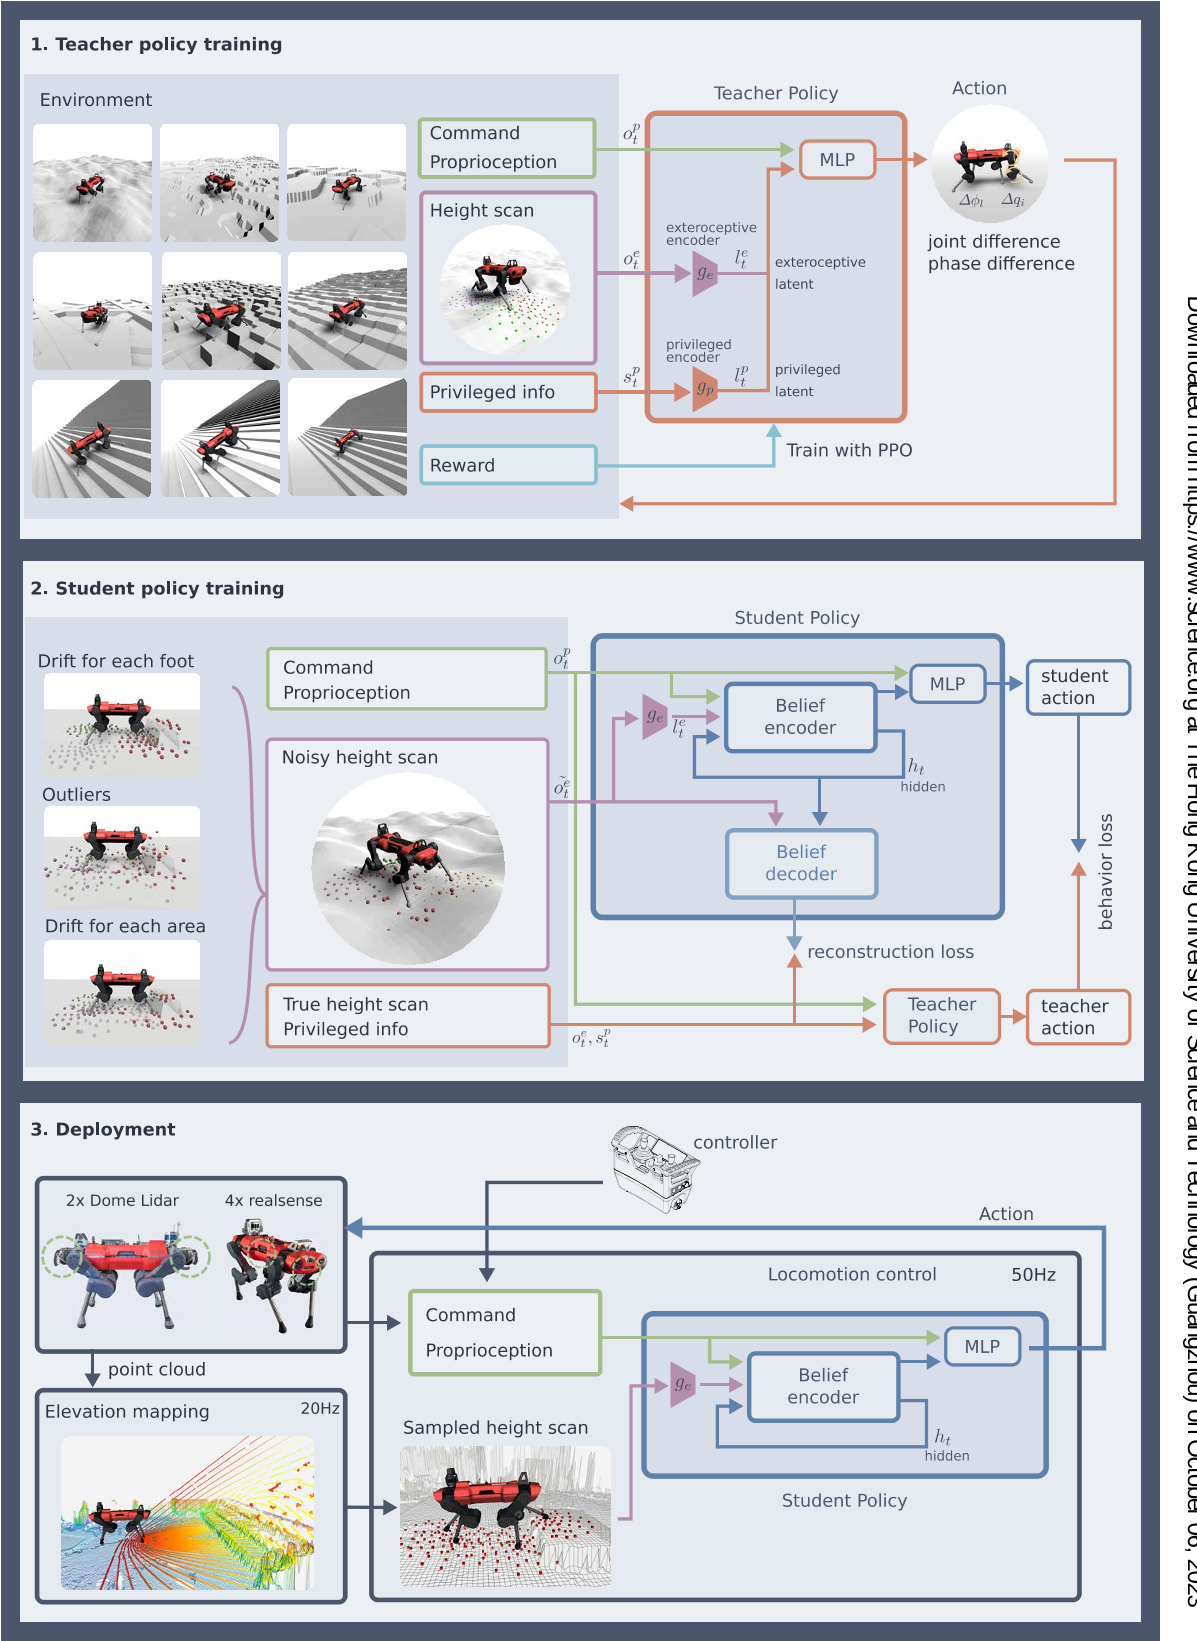
\includegraphics[width=1.0\linewidth]{train_process.png}
  \caption{RL implementation process\cite[p9]{Miki_Lee_Hwangbo_Wellhausen_Koltun_Hutter_2022}.}
  \label{fig:process}
\end{figure}

% \textcolor{gray}{\small 这节主要参考文献\cite[p10-12]{Miki_Lee_Hwangbo_Wellhausen_Koltun_Hutter_2022}。}

整个神经网络的训练是在仿真环境中完成的,然后采用\emph{zero-shot sim-to-real}的转换部署到实际的额机器人上。整个方法分为三个阶段,如图\ref{fig:process}所示。
\begin{enumerate}
  \item 首先,使用RL训练教师策略,以在随机生成的具有随机干扰的地形上遵循随机目标速度。该策略可以访问特权信息,例如无噪声地形测量、地面摩擦和引入的扰动。
  \item 在第二阶段,训练学生策略重现教师策略的动作,而不使用这种特权信息。学生策略构造一个信念状态来使用循环编码器捕获未观察到的信息,并根据该信念状态输出一个动作。在训练期间,我们利用两个损失:\emph{行为克隆损失}和\emph{重建损失}。行为克隆损失旨在模仿教师策略。重新构造损失鼓励编码器产生信息丰富的内部表示。
  \item 最后,我们将学习到的学生策略转移到物理机器人上,并将其与机载传感器在现实世界中部署。机器人通过整合来自板传感器的深度数据和从构建的高程图中采样高度读数来构建高程图,以形成策略的外部感知输入。这种外部感知输入与本体感觉数据相结合,并提供给神经网络,该网络产生执行器命令。\emph{板上传感器和自身构建等高图融合}
\end{enumerate}

\subsection[问题描述]{问题描述}

我们在离散时间动力学中制定了我们的控制问题,其中环境完全由时间步$t$的状态$s_t$定义。该策略实施一个动作$a_t$并且从环境中获得一个观测结果$o_t$,这个测量结果来自观测模型$\mathcal{O}(o_t|s_t,a_t)$。接着环境以$P(s_{t+1}|s_t, a_t)$的概率转移到下一个状态$s_{t+1}$并给出一个奖励$r_{t+1}$。

当所有状态都可以被观测的实况下,也即$o_t=s_t$时,整个问题可以被看做一个马尔可夫决策过程\emph{Markov decision process(MDP)}。然而,当存在不可观察性的信息时,例如外力或完整的地形信息,动力学被建模为部分可观察的马尔可夫决策过程\emph{partially observable Markov decision process(POMDP)}。

RL的目标是找到一个能够使得未来轨迹的预期折扣奖励最大化的策略$\mathbfit{\pi}^*$,以使得:
\begin{align}
  \mathbfit{\pi}^*=\underset{a}{argmax}E[\sum_{t=0}^{\infty}\gamma^t r_t]
\end{align}

已经开发了许多RL算法来解决完全可观察的MDP问题,并且易于用于训练。然而,POMDP问题的情况更具挑战性,因为状态不能完全观察到。这通常通过从历史的观察结果$o_0, \cdots, o_t$中构建一个信念状态$b_t$\emph{belief state}以尝试构建完全状态的方式来解决。在深度RL中,这通常是通过堆叠一系列先前的观察结果\cite[p]{Mnih_Kavukcuoglu_Silver_Graves_Antonoglou_Wierstra_Riedmiller_2013}或使用可以压缩过去信息的架构来完成的,例如循环神经网络 (RNN) \cite[p]{Zhu_Li_Poupart_Miao_2017}或时间卷积网络\cite[p]{Lee_Hwangbo_Wellhausen_Koltun_Hutter_2020,Bai_Kolter_Koltun_2018}。

从头开始训练一个天真地处理序列数据的复杂的神经网络策略可能很耗时\cite[p]{Lee_Hwangbo_Wellhausen_Koltun_Hutter_2020}。因此,我们使用特权学习(45),我们首先训练一个具有特权信息的教师策略,然后通过监督学习将教师策略提炼为学生策略\cite[p]{Chen_Zhou_Koltun_Krähenbühl_2019}。

\begin{enumerate}
  \item 训练环境:
  \item 地形:
  \item 域随机化:
  \item 片段终止条件:
\end{enumerate}

\subsection[教师策略训练]{教师策略训练}

在训练的第一阶段,我们的目标是找到一个可以访问完美、特权信息的最佳参考控制策略,并使ANYmal在随机生成的地形上遵循所需的命令速度。命令需求随机生成并构成一个向量$\mathbfit{v}_des\in \mathbb{R}^3=(v_x,v_y,w)$,其中$v_x, v_y$分别表示在机器人自身坐标系下的纵向速度和横向速度,$w$表示自转速度。

我们采用近端策略优化\emph{proximal policy optimization(PPO)}\cite[p]{Schulman_Wolski_Dhariwal_Radford_Klimov_2017}来训练教师策略。教师策略被建模为一个高斯策略,$a_t~\mathcal{N}(\pi_{\theta}(o_t=s_t),\sigma I)$,其中$\pi_{\theta}$由用$\theta$参数化的多层感知器\emph{multilayer perceptron(MLP)}实现,$\sigma$表示每个动作之间的方差。

\subsection[观测和行动]{观测和行动}

教师策略的观察定义为$o_t^{teacher}=(o_t^p, o_t^e, s_t^p)$,其中$o_t^p$表示本体感觉观察\emph{proprioception observation},$s_t^e$表示外部观察\emph{exteroceptive observation},$s_t^p$表示特权状态\emph{privileged state}。
\begin{itemize}
  \item $o_t^p$包含本体速度、转动、节点位置和速度历史、动作历史、每条腿的相位;
  \item $o_t^e$是每只脚周围高度样本的向量,包括五种不同的半径;
  \item $s_t^p$包括接触状态、接触力、接触法线、摩擦系数、大腿和小腿接触状态、施加到身体上外部力和力矩、摆动阶段持续时间;
\end{itemize}

我们的动作空间受到中心模式生成器的启发\cite[p]{Lee_Hwangbo_Wellhausen_Koltun_Hutter_2020}。每条腿$l={1,2,3,4}$保存一个相位变量$\phi_l$并定义了基于相位的标称轨迹。这个标称轨迹是一个脚尖的步进运动,我们使用逆运动学来计算每个关节执行器$i={1, \dots, 12}$的标称关节目标$q_i(\phi_l)$。来自策略的动作是相差$\Delta \phi_l$和关节位置目标残差$\Delta q_i$。\textcolor{gray}{\small 更详细相关内容看相关附件的S5。}

\subsection[策略构架]{策略构架}

我们将教师策略$\pi_{\theta}$建模为一个MLP。它包括三个MLP组成部分:外部感知编码器、特权编码器、主网络,如图\ref{fig:process}所示。
\begin{enumerate}
  \item 外部感知编码器$g_e$接收来自$o_t^e$的信息,然后输出一个小些的潜在表示$$l_t^e=g_e(o_t^e)$$
  \item 特权编码器$g_p$接收来自特权状态$s_t^p$的信息,然后输出一个潜在表示$$l_t^{priv}=g_p(s_t^p)$$
  \item 
\end{enumerate}

这些编码器将每个输入压缩为更紧凑的表示,并使得学生策略能更方便地重用一些教师策略组件。\textcolor{gray}{\small 更详细相关内容看相关附件的S6。}

\subsection[奖励函数]{奖励函数}

针对速度控制命令的跟随,我们定义正奖励;针对违反约束的情况,我们定义负奖励。指令跟随奖励定义如下:
\begin{align}
  \mathbfit{r}_{command}=\begin{cases}
    1.0, &if \mathbfit{v}_{des}\cdot\mathbfit{v}>|\mathbfit{v}_{des}|\\
    \exp(-(\mathbfit{v}_{des}\cdot\mathbfit{v})^2), &otherwise
  \end{cases}
\end{align}

其中$\mathbfit{v}_{des}\in\mathbb{R}^2$是所需的水平速度,$\mathbfit{v}\in\mathbb{R}^2$是身体坐标系下当前身体速度。同样的奖励机制也被应用与转动速度情况。

我们惩罚与期望速度正交的速度分量以及横摇、俯仰和偏航周围的身体速度。此外,我们使用整形奖励进行身体方向、关节扭矩、关节速度、关节加速度和脚滑以及小腿和膝盖碰撞。身体方向奖励用于避免身体的奇怪姿势。联合相关奖励术语用于避免过于激进的运动。脚滑和碰撞奖励术语用于避免它们。我们通过在模拟中查看策略的行为来调整奖励术语。除了遍历性能外,我们还检查了运动的平滑度。
\textcolor{gray}{\small 更详细相关内容看相关附件的S7。}

\subsection[课程]{课程}
随着策略性能的提高,我们使用两个课程来提高难度。
一个课程使用自适应方法\cite[p]{Lee_Hwangbo_Wellhausen_Koltun_Hutter_2020}调整地形难度,另一个改变元素,如奖励或使用逻辑函数\cite[p]{Hwangbo_Lee_Dosovitskiy_Bellicoso_Tsounis_Koltun_Hutter_2019}应用干扰。

对于地形课程,粒子滤波更新地形参数,使它们仍然具有挑战性,但在策略训练期间的任何时候都可以实现\cite[p]{Lee_Hwangbo_Wellhausen_Koltun_Hutter_2020}。

第二个课程将域随机化的幅度和一些奖励项(关节速度、关节加速度、方向、滑移和大腿和小腿接触)乘以单调递增且渐近趋势为 1 的因子:$$c_{k+1}=(c_k)^d$$

其中$c_k$是第$k$次迭代的课程因子,$d\in(0,1)$是收敛率。

\subsection[学生策略训练]{学生策略训练}

在我们训练好一个可以在特权信息的帮助下穿越各种地形教师策略后,我们就可以将其提炼成一个学生策略,该策略只能访问真实robot上可用的信息。我们使用与教师策略相同的训练环境,但在学生高度样本观察中添加额外的噪声:$o_t^{student}=(o_t^p,n(o_t^e))$,其中$n(o_t^e)$是一个用于高度样本输入的噪声模型。该噪声模型模拟了现场部署过程中经常遇到的外部感觉的不同失败案例,具体如下。

当外部感觉中存在较大的噪声时,它变得不可观察;因此,动力学被认为是POMDP。此外,由于缺乏直接测量的传感器,特权状态是不可观察的。因此,该策略需要考虑顺序相关性来估计不可观察的状态。我们建议使用\emph{循环信念状态编码器}来组合外部感知和本体感觉的序列,以估计不可观察的状态作为信念状态。

学生策略由循环信念状态编码器和MLP组成,如图\ref{fig:process}所示。我们用$h_t$表示循环网络的隐藏状态。信念状态编码器接收$o_t^{sutdent},h_t$并输出一个潜在向量$b_t$,它表示信念状态。我们的目标是将信念状态$b_t$与编码所有运动相关信息的教师策略的特征向量($l_t^e, l_t^{priv}$)进行匹配。
接下来我们将$o_t^p$和$b_t$传入MLP,由它计算出最终的动作。MLP结构与教师策略相同,这样我们就可以重用教师策略的学习权重来初始化学生网络并加快训练速度。

学生策略的训练通过最小化两个损失以有监督的方式进行训练:行为克隆损失\emph{behavior cloning loss}和重建损失\emph{reconstruction loss}。
\begin{itemize}
  \item 克隆损失定义为给定相同状态和指令的学生动作和教师动作之间的平方距离。
  \item 重建损失定义为无噪声高度样本和特权信息($o_t^e, s_t^p$)及其与信念状态$b_t$的重建之间的平方距离。
\end{itemize}

我们通过推出学生策略来生成样本,以提高鲁棒性\cite[p]{Ross_Gordon_Bagnell_2010,Czarnecki_Pascanu_Osindero_Jayakumar_Swirszcz_Jaderberg_2019}。

\subsection[高度采样随机化]{高度采样随机化}

\begin{figure}
  \centering
  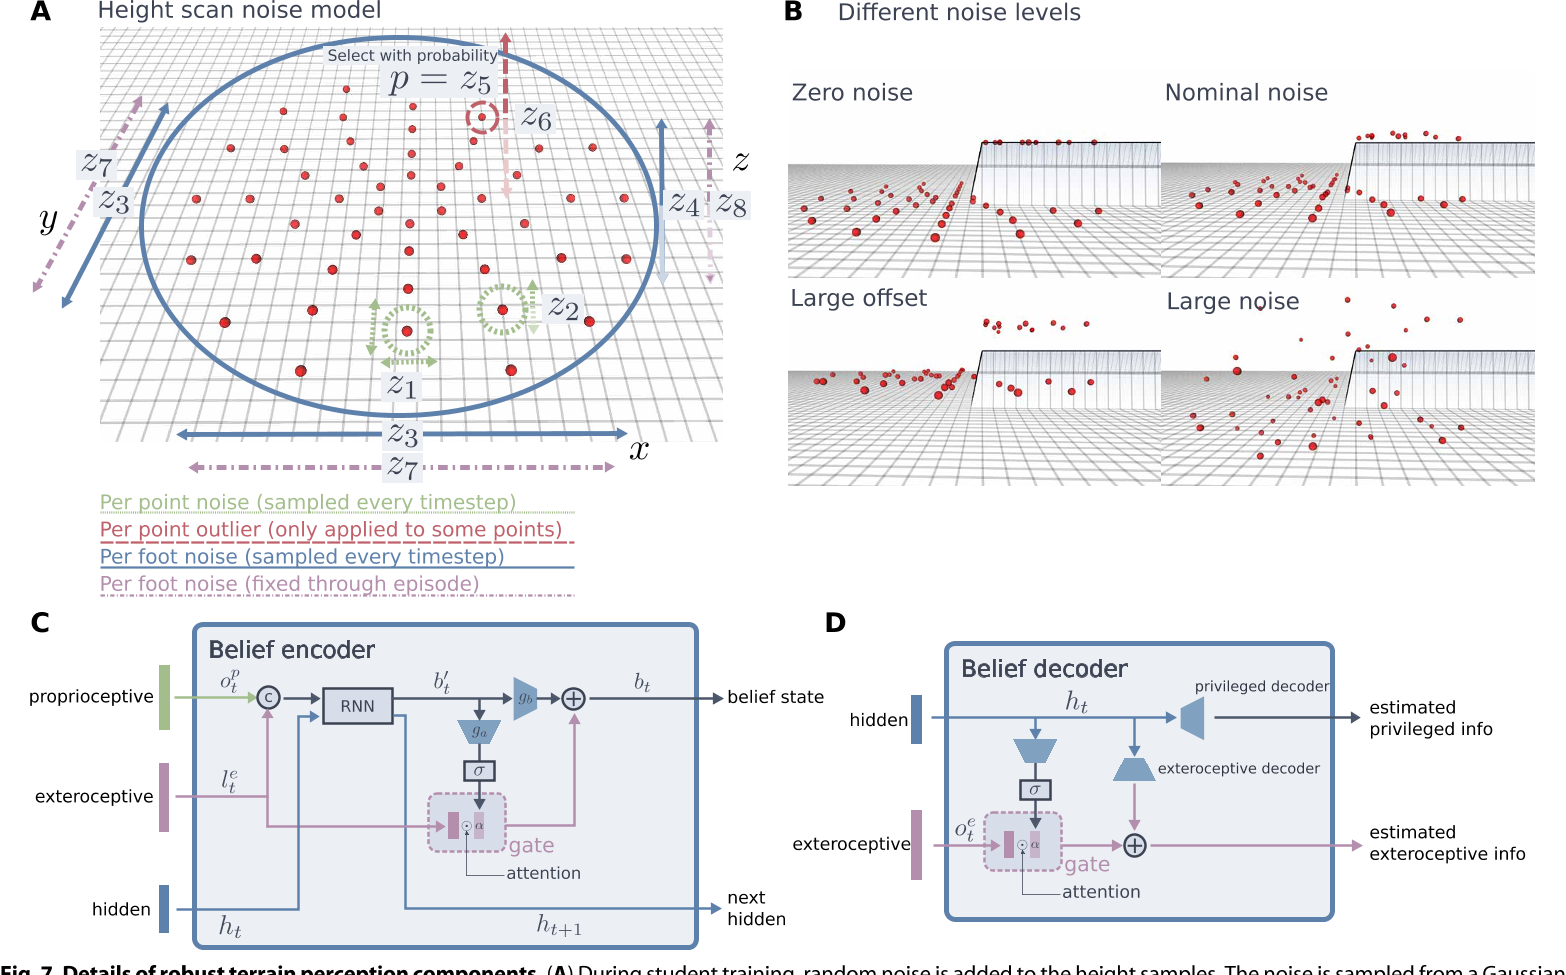
\includegraphics[width=1.0\linewidth]{terrain_perception.png}
  \caption{Robust terrain perception\cite[p10]{Miki_Lee_Hwangbo_Wellhausen_Koltun_Hutter_2022}.}
  \label{fig:terrain_perception}
\end{figure}

在学生训练过程中,我们使用参数化噪声模型$n(\sigma_t^e|o_t^e,z),z\in \mathbb{R}^{8\times 4}$将随机噪声注入到高度样本中。
我们在对高度进行采样时应用了两种不同类型的测量噪声,如图\ref{fig:terrain_perception}A所示:
\begin{enumerate}
  \item 横向移动扫描点。
  \item 扰动高度值。
\end{enumerate}

每个噪声值都是从高斯分布中采样的,噪声参数$z$定义方差。这两种类型的噪声都应用于三个不同的范围,所有这些都有自己的噪声方差:每个扫描点、每只脚和每一集。每个扫描点和每只脚的噪声值在每个时间步重新采样,而所有扫描点的表观轮廓噪声保持不变。

此外,我们定义了三个具有相关噪声参数$z$的映射条件来模拟不断变化的地图质量和误差源,如图\ref{fig:terrain_perception}B所示。
\begin{enumerate}
  \item 名义噪声假设常规操作期间具有良好的地图质量。
  \item 大偏移量噪声来模拟由于姿态估计漂移或可变形地形造成的地图偏移。
  \item 幅度较大的噪声来模拟由于遮挡或映射失败导致完全缺乏地形信息的情况。
\end{enumerate}

这三个映射条件在每个训练集的开头以60、30和10\%的比例选择。

最后,我们将每个训练地形划分为单元格,并向高度样本添加附加偏移量,具体取决于它采样的单元格。这模拟了不同地形特征的区域之间的转换,如植被和深度雪。参数向量$z$也是学习课程的一部分,其幅度随训练持续时间线性增加。

\textcolor{gray}{\small 更详细相关内容看相关附件的S8。}

\subsection[信念状态寄存器]{信念状态寄存器}

循环信念状态编码器编码不能直接观察到的状态。为了整合本体感受和外感受数据,我们引入了一个门控编码器,如图 7C 所示,灵感来自门控 RNN 模型\cite[p]{Cho_van_Merrienboer_Gulcehre_Bahdanau_Bougares_Schwenk_Bengio_2014,Hochreiter_Schmidhuber_1997}和多模态信息融合 (4-66)。

信念状态编码器学习使用一个可变的门控因子来控制外部感知信息通过的量。首先,内部感知$s_t^p$、从含噪声观测提取的外部感知$l_t^e=g_e(\widetilde o_t^e)$以及隐藏状态$s_t$被RNN模型编码成为一个中间信念状态$b_t{t'}$。它控制最终进入$b_t$的外部感知信息量:
\begin{align}
  b_{t'},h_{t+1}=RNN(o_t^p,l_t^e,h_t)\\
  \alpha = \sigma (g_a(b_{t'}))\\
  b_t = g_b(b_{t'})+l_t^e \odot \alpha
\end{align}

这里$g_a,g_b$是全连接的神经网络,$\sigma(\cdot)$是sigmoid函数。

解码器使用相同的门,用于重建特权信息和高度样本(图 7D)。这用于计算重建损失,它鼓励信念状态捕获有关环境的真实信息。我们使用 GR\cite[p]{Cho_van_Merrienboer_Gulcehre_Bahdanau_Bougares_Schwenk_Bengio_2014}作为我们的 RNN 架构。

\textcolor{gray}{门结构有效性的评估见第 S9 节。}

\subsection[部署]{部署}

我们在 PyTorch\cite[p]{Paszke_Gross_Massa_Lerer_Bradbury_Chanan_Killeen_Lin_Gimelshein_Antiga_et_al_2019}中训练策略,并在没有任何微调的情况下部署在机器人 zero-shot上。我们通过估计机器人的姿态,并相应地从传感器中调节点云读数,构建了一个以机器人为中心的2.5D高程图刷新率为20赫兹。该策略以50Hz运行,并从最新的高程图中映射采样高度;如果查询位置没有可用的地图信息,则填充随机采样的值。

我们开发了一个高程映射管道,用于在图形处理单元上快速地形映射,以并行化点云处理。我们遵循与Fankhauser等人\cite[p]{Fankhauser_Bloesch_Hutter_2018}使用的类似方法,以卡尔曼滤波的方式更新地图,另外按漂移补偿\emph{drift compensation}和光线投射\emph{ray casting}以获得更吻合的地图。这种快速映射实现对于保持快速处理速率和跟上我们的控制器实现的快速运动速度至关重要。


% !TeX root = ../sustechthesis-example.tex

\chapter{RL控制框架分析}

这部分将分析不同类型的RL控制实现框架。一般来说对机器人的控制不仅需要一个良好训练后的策略,还需要一些外围的辅助模块。因为机器人控制的直接控制目标是关节点,而很多RL策略给出的并不是直接可以对应到关节点位置、扭矩等的信息,而是以残差控制的形式给出的。首先机器人自己会有一套基础的轨迹生成器(中心模式生成器)及相应的电机闭环控制,RL策略起作用的方式是给中心模式生成器的结果进行额外的调整再输入给电机,也就是残差控制。

\section[RL案例1]{Learning quadrupedal locomotion over challenging terrain\cite[p7]{Lee_Hwangbo_Wellhausen_Koltun_Hutter_2020}}

\subsection[总体概况]{总体概况}

\begin{figure}
    \centering
    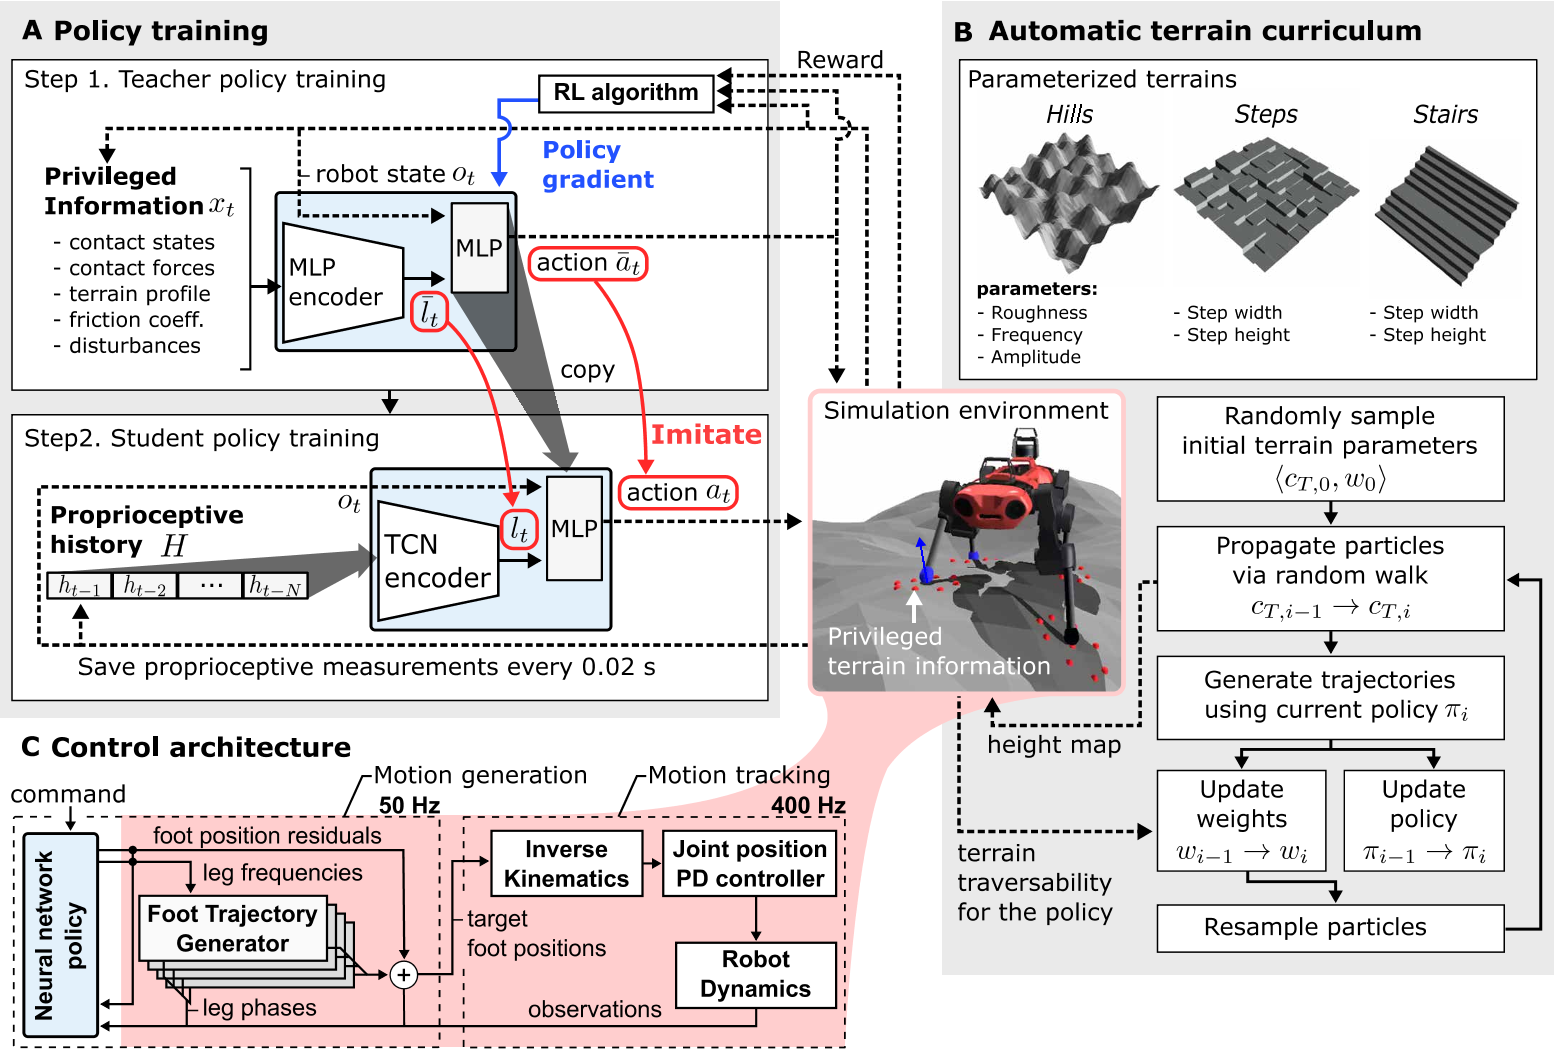
\includegraphics[width=1.0\linewidth]{creating_a_proprioceptive_locomotion_controller.png}
    \caption{Creating a proprioceptive locomotion controller\cite[p7]{Lee_Hwangbo_Wellhausen_Koltun_Hutter_2020}.}
    \label{fig:creating_a_proprioceptive_locomotion_controller}
  \end{figure}

  图\ref{fig:creating_a_proprioceptive_locomotion_controller}是一个只采用本体感知进行机器狗控制的RL策略实现架构。它包括训练定义、地形定义、控制架构。
  \begin{itemize}
    \item 策略训练:整个RL训练采用\emph{特权训练(privileged training)}\cite[p]{Chen_Zhou_Koltun_Krähenbühl_2019}的理念,训练过程分为两个阶段,如图\ref{fig:creating_a_proprioceptive_locomotion_controller}A所示。第一阶段用完善的特权信息作为输入训练出一个\emph{教师策略(teacher policy)};第二阶段仅用本体感知作为输入训练出一个\emph{学生策略(student policy)},学生策略的训练过程通过模仿教师策略实现。实际部署到机器人上的策略是学生策略。
    \item 地形定义:RL训练过程是在一定的地形条件下完成的,如图\ref{fig:creating_a_proprioceptive_locomotion_controller}B所示。对于同样的控制命令,不同的地形条件会产生不同的任务难度。为了能更好地促进训练进步,训练过程中的地形采用\emph{自适应地形课程(adaptive terrain curriculum)},它会从简单地形开始根据训练控制器的性能提升而不断提高地形难度,使得RL控制器时钟面对相对于当前状况的中等地形难度。
    \item 控制架构:整个控制架构采用\emph{调节轨迹生成器(Policies Modulating Trajectory Generators, PMTG)\cite[p]{Iscen_Caluwaerts_Tan_Zhang_Coumans_Sindhwani_Vanhoucke_2018}}架构来提供运动生成的先验。神经网络策略通过合成残差位置命令来调节腿相和运动原语,如图\ref{fig:creating_a_proprioceptive_locomotion_controller}C所示。
  \end{itemize}


\subsection[策略训练]{策略训练}
\subsubsection[教师策略]{教师策略}
整个控制问题被构建成一个\emph{马尔科夫决策过程(Markov Decision Process, MDP)}。MDP是一种用于状态和结果部分随机的离散时间控制过程的数学框架。MDP被定义为一个状态空间$\mathcal{S}$,动作空间$\mathcal{A}$,一个标量奖励函数$\mathcal{R}(s_t,s_{t+1})$,一个转移概率$P(s_{t+1}s_t, a_t)$。一个学习代理从策略$\mathbfit{\pi}(a_t|s_t)$中选择一个动作$a_t$并从环境中获得奖励$r_t$。RL的目的是找到一个优化的策略$\mathbfit{\pi}^*$使得无限时间范围内的折扣奖励总和最大。

状态空间$s_t$定义为:$\langle o_t, x_t\rangle$,其中$o_t$是机器人自身的观测信息,$x_t$是特权信息。
\begin{align}
    s_t\begin{cases}
        o_t\begin{cases}
            proprioceptive\ sensors\\
            state\ estimator\begin{cases}
                base\ velocity\\
                orientation\\
            \end{cases}\\
        \end{cases}\\
        x_t\begin{cases}
            only\ for\ simulation
        \end{cases}\\
    \end{cases}
\end{align}

动作空间$\overline a_t$是一个16维向量,由腿的频率和交的位置残差构成。

奖励函数$\mathcal{R}(s_t|s_{t+1})$定义。

\textcolor{red}{reward function definition details ...}

如图\ref{fig:creating_a_proprioceptive_locomotion_controller}A所示,策略网络由两个MLP模块构成。
第一个MLP模块将$x_t$信息转化成潜在向量$\overline{l}_t$,由于$x_t$中并不含有机器人的状态或指令信息,也就是说他只包含地形信息和接触相关的信息。假设$\overline{l}_t$的作用是驱动自适应行为,比如根据地形轮廓改变脚步间隙大小。然后$\overline{l}_t$和$o_t$再提供给第二个MLP网络来计算动作。

训练采用\emph{信任区域策略优化(Trust Region Policy Optimization, TRPO)}\cite[p]{Schulman_Levine_Moritz_Jordan_Abbeel_2015}。

\subsubsection[学生策略]{学生策略}

学生策略仅能获取$o_t$信息。这里的一个关键假设是潜在特征$\overline{l}_t$可以从本体感觉观察的时间序列$h_t$中恢复(部分),$h_t:=o_t\{f_o, joint\ history, previous\ foot\ position\ targets \}$。

学生策略采用TCN\cite[p]{Bai_Kolter_Koltun_2018}编码器。使用TCN架构的原因是它对输入历史长度提供透明的控制,可以容纳长历史,并且已知对超参数设置具有鲁棒性\cite[p]{Bai_Kolter_Koltun_2018}。

学生策略采用监督学习的方式进行训练,损失函数定义为:
\begin{align}
    \mathcal{L}:=(\overline{a}_t(o_t,x_t)-a_t(o_t,H))^2+(\overline{l}_t(o_t, x_t)-l_t(H))^2
\end{align}
带$(\overline{\cdot})$标识的项是来自教师策略的生成。对于每个访问的状态,教师策略计算其嵌入和动作向量$(\overline{\cdot})$,这些教师策略的输出随即被用作与相应状态相关的监督信号。


\subsection[地形定义]{地形定义}
\textcolor{red}{Adaptive terrain curriculum ...}

\subsection[控制架构]{控制架构}

整个控制架构结构如图\ref{fig:creating_a_proprioceptive_locomotion_controller}C所示。它被分为两大类:\emph{运动生成}、\emph{跟随}。整个系统的输入只有\emph{控制指令}和\emph{本体感知},输出为\emph{关节点位置目标}。

运动生成策略是一种基于周期性腿相位的策略,之前的一些工作中通常利用预定义的脚接触时间表\cite[p7]{Bellicoso_Jenelten_Gehring_Hutter_2018,Barasuol_Buchli_Semini_Frigerio_De_Pieri_Caldwell_2013}。为每条腿都定义一个周期的相位变量$\phi_i\in[0.0,2\pi)$。在每一个时间步长$t$里,$\phi_i = (\phi_{i,0}+(f_0+f_i)t)(\mod 2\pi)$,其中$\phi_{i,0}$是初始相位,$f_0$是一般基础频率,$f_i$是第$i$条腿的频率偏移。我们希望腿在$f_0+f_i\neq 0$时表现出周期性运动,并在接触阶段与地面接触。这里基础频率参考之前开发的传统控制\cite[p7]{Bellicoso_Jenelten_Gehring_Hutter_2018}中鹦鹉步态的值,$f_0=1.25$Hz。

\textcolor{red}{target foot position...}

我们采用PMTG架构来将神经网络集成系统中用来调节控制器的输出。整体实现由四个完全相同的\emph{足迹生成器(foot trajectory generators, FTGs)}和一个\emph{神经网络策略(neural network policy, NNP)}构成。足迹生成器是一个输出每条腿的脚位置的函数:$F(\phi):[0.0,2\pi)\to \mathbb{R}^3$。这个FTG在$f_i$不为零时驱动垂直方向的踱步运动。
\textcolor{gray}{\small
$F(\phi)$的定义如下:
\begin{align}
    F(\phi_i)=\begin{cases}
        (h(-2k^3+3k^2)-0.5)^{H_i}z &k\in[0,1]\\
        (h(2k^3-9k^2+12k-4)-0.5)^{H_i}z &k\in[1,2]\\
        -0.5^{H_i}z & otherwise\\
    \end{cases}
\end{align}
其中$k=2(\phi_i-\pi)/\pi$,$h$是一个表示最大步高的参数。在摆动相位的每一个阶段都是一个连接最高点和最低点的三次Hermite样条曲线,在连接点处曲线具有一阶连续性(一阶导数为零)。其它的周期函数,如$h_i \sin (\phi_i)$可以用于FTG。给定一组合适的$f_0,h,\phi_{i,0}$参数值,机器人就能稳定地在地面上踱步了。比如,文献\cite[p7]{Lee_Hwangbo_Wellhausen_Koltun_Hutter_2020}中使用的值:$f_0=1.25,h=0.2$,$\phi_{i,0}$从$U(0,2\pi)$中采样得到。}
神经网络策略输出$f_{iS}$和脚的目标位置残差($\Delta \mathbfit{r}_{f_i, T}$)。这样,第$i$个脚的目标位置是$\mathbfit{r}_{f_i, T}:=F(\phi_i)+\Delta \mathbfit{r}_{f_i, T}$。

跟随控制是使用解析\emph{逆运动学(inverse kinematics, IK)}和关节点\emph{位置控制(position control)}实现的。在$H_i$中定义的脚位置首先表述在机器人身体系中,然后用IK计算关节点的位置目标。而关节点的位置目标依靠关节点的PD控制器来跟随。使用IK的好处是可以最大化计算效率同时在\emph{仿真到实际(sim-to-real)}的过程中可以复用已有的位置控制驱动器模型\cite[p]{Lee_Hwangbo_Hutter_2019,Hwangbo_Bellicoso_Fankhauser_Huttery_2016}。


% 结论
\backmatter
% !TeX root = ../sustechthesis-example.tex

\begin{conclusion}

学位论文的结论作为论文正文的最后一章单独排写,但不加章标题序号。

结论应是作者在学位论文研究过程中所取得的创新性成果的概要总结,不能与摘要混为一谈。博士学位论文结论应包括论文的主要结果、创新点、展望三部分,在结论中应概括论文的核心观点,明确、客观地指出本研究内容的创新性成果(含新见解、新观点、方法创新、技术创新、理论创新),并指出今后进一步在本研究方向进行研究工作的展望与设想。对所取得的创新性成果应注意从定性和定量两方面给出科学、准确的评价,分(1)、(2)、(3)…条列出,宜用“提出了”、“建立了”等词叙述。

\end{conclusion}



% 参考文献
\bibliography{ref/refs, ref/appendix}  % 参考文献使用 BibTeX 编译
% \bibliography{ref/appendix}  % 参考文献使用 BibTeX 编译
% \printbibliography       % 参考文献使用 BibLaTeX 编译(兼容性不佳,不太推荐)

% % 附录
% \appendix
% % !TeX root = ../sustechthesis-example.tex








\chapter{补充内容}

在附录里面我会写一些控制相关的一些数学概念的理解。

% ==============================================================================
\section{拉格朗日乘子法}

在机械狗的运动规划中,机械狗质心的运动是通过求解空间中$x, y, z$方向上的五次曲线得到的。这个五次曲线是在一些列约束条件下的最优运动结果。这个结果是通过求解QP(二次优化)问题得到的。实际上所谓的QP问题的一种形式就是之前高数上很熟悉的`拉格朗日乘子法(Lagrange Multiplier)'。下面就对这部分知识进行总结,这部分内容主要参考\href{https://juejin.cn/post/6956879956299218974}{这个博客}。




\subsection{优化问题}

通常我们需要求解的优化问题有如下几类:
\begin{enumerate}
  \item 无约束优化问题,可以写为:\begin{align*}
    &min f(x);
  \end{align*}
  \item 有等式约束的优化问题,可以写为:\begin{align*}
    &min f(x); \\ 
    &s.t. \quad h_i(x)=0, i = 1, \dots, n;
  \end{align*}
  \item 有等式和不等式约束的优化问题,可以写为:\begin{align*}
    &min f(x); \\
    &s.t. \quad g_i \leq 0, i = 1, \dots, n; \\
    &and \quad h_i(x)=0, i = 1, \dots, n;
  \end{align*}
\end{enumerate}

对于第一类优化问题,常使用的求解方式是\emph{Fermat定理},即使用求取$f(x)$的导数,然后令其为零,可以求得候选的最优值,再在这些候选值中验证;如果是凸函数,可以保证是最优解。

对于第二类优化问题,常使用的求解方式是\emph{拉格朗日乘子法},即把等式约束$h_i(x)$用一个系数与$f(x)$写为一个式子,称为`拉格朗日函数',而系数称为拉格朗日乘子。通过拉格朗日函数对各个变量求导,令其为零,可以求得候选值集合,然后验证求得最优值。

对于第三类优化问题,常使用的求解方式是\emph{KKT}条件。同样地,把所有等式、不等式约束条件与$f(x)$写成一个式子,也叫拉格朗日函数,系数也称为拉格朗日乘子。通过一些条件可以求出最优值的必要条件,这个条件称为KKT条件。




\subsection{拉格朗日乘子法}
对于等式约束,我们可以通过一个拉格朗日系数$a$把等式约束和目标函数组合成一个拉格朗日函数:
\begin{align}
  \mathbfit{L}(\mathbfit{a},\mathbfit{x})=\mathbfit{f}(\mathbfit{x})+\mathbfit{a}\mathbfit{h}(\mathbfit{x})
\end{align}

其中$\mathbfit{a},\mathbfit{h}(\mathbfit{x})$分别为一行向量和列向量。最优值可以通过对拉格朗日函数$\mathbfit{L}(\mathbfit{a},\mathbfit{x})$的各个参数求导取零,联立等式进行求取。它要求:
\begin{enumerate}
  \item 拉格朗日函数对$\mathbfit{a}$的偏导为零,即$\frac{\partial\mathbfit{L}(\mathbfit{a},\mathbfit{x})}{\partial \mathbfit{a}}=0$;
  \item 拉格朗日函数对$\mathbfit{x}$的偏导为零,即$\frac{\partial\mathbfit{L}(\mathbfit{a},\mathbfit{x})}{\partial \mathbfit{x}}=0$;
\end{enumerate}

通过联立求解上面两个条件等式可以求得候选的最优值结果$\mathbfit{a},\mathbfit{x}$的候选值,然后验证$\mathbfit{x}$求得最优值(如果是如函数可以保证是最优解)。




\subsection{KKT条件}
对于含有不等式约束的优化问题,常用的方法是KKT条件同样像等式约束一样将所有的不等约束也添加到拉格朗日函数中谢伟一个式子:
\begin{align}
  \mathbfit{L}(\mathbfit{a},\mathbfit{b},\mathbfit{x})=\mathbfit{f}(\mathbfit{x})+\mathbfit{a}\mathbfit{g}(\mathbfit{x})+\mathbfit{b}\mathbfit{h}(\mathbfit{x})
\end{align}

KKT条件指出最优值必须满足一下三个条件:
\begin{enumerate}
  \item 拉格朗日函数对$x$求导为零,即$\frac{\mathbfit{L}(\mathbfit{a},\mathbfit{b},\mathbfit{x})}{\partial \mathbfit{x}}$;
  \item 等式约束自身为零,即$\mathbfit{h}(\mathbfit{x})=0$;
  \item 不等约束及其系数乘积为零,即$\mathbfit{a}\mathbfit{g}(\mathbfit{x})=0$;
\end{enumerate}

求取这三个等式之后就能得到候选最优值。其中第三个式子非常有趣,因为$\mathbfit{g}(\mathbfit{x})\leq 0$,如果要满足这个等式,必须$\mathbfit{a}=0$或者$\mathbfit{g}(\mathbfit{x})= 0$. 这是\emph{SVM}的很多重要性质的来源,如支持向量的概念。







% ==============================================================================
\section{二次规划问题}

二次规划(QP, Quadratic Programming)定义:目标函数为二次函数,约束条件为线性约束,属于最简单的一种非线性规划。这部分内容主要参考\href{https://zhuanlan.zhihu.com/p/375762164}{这个博客}。




\subsection{等式约束的QP问题}

一个标准的等式约束QP问题模型如下:
\begin{align}
  &min \quad \frac{1}{2}\mathbfit{x}^T\mathbfit{H}\mathbfit{x}+\mathbfit{g}^T\mathbfit{x} \notag\\
  &s.t. \quad \mathbfit{a}_i^T\mathbfit{x}=b_i, \quad i = 1, 2, \dots, m
\end{align}

其中$\mathbfit{H}$是由二阶导构成的Hessian矩阵,$\mathbfit{g}^T\mathbfit{x}$是由梯度构成的Jacobi矩阵,这里的向量都是列向量,$\mathbfit{g}^T\mathbfit{x}$表示转置成行向量。

其对应的拉格朗日函数为:
\begin{align}
  \mathbfit{L}(\mathbfit{x},\mathbfit{\lambda})=\frac{1}{2}\mathbfit{x}^T\mathbfit{H}\mathbfit{x}+\mathbfit{g}^T\mathbfit{x}+\sum_{i=1}^{m}\lambda_i(\mathbfit{a}_i^T\mathbfit{x}-b_i)
\end{align}

满足KKT条件,即满足:
\begin{align}
  \begin{cases}
    \frac{\partial \mathbfit{L}}{\partial \mathbfit{x}}=\mathbfit{H}\mathbfit{x}+\mathbfit{g}+\sum_{i=1}^{m}\lambda_i\mathbfit{a}_i=0\\
    \frac{\partial \mathbfit{L}}{\partial \lambda_i}=\mathbfit{a}_i^T\mathbfit{x}-b_i=0, \quad i = 1, 2, \dots, m
  \end{cases}
\end{align}

将其写成矩阵形式:
\begin{align}
  \mathbfit{F}(\mathbfit{x},\mathbfit{\lambda})=\begin{bmatrix}
    \mathbfit{H}\mathbfit{x}+\mathbfit{g}+\mathbfit{\lambda}\mathbfit{a}\\
    \mathbfit{a}^T\mathbfit{x}-\mathbfit{b}
  \end{bmatrix} = 0
\end{align}

其中
\begin{align}
  \mathbfit{\lambda}=\begin{bmatrix}
    \lambda_1 & 0 & \dots & 0\\
    0 & \lambda_2 & \dots & 0\\
    \vdots & \vdots &\ddots & \vdots\\
    0 & 0 &\dots & \lambda_m
  \end{bmatrix}, \quad
  \mathbfit{a}^T=\begin{bmatrix}
    \mathbfit{a}_1^T \\ \mathbfit{a}_2^T \\ \vdots \\ \mathbfit{a}_m^T
  \end{bmatrix}, \quad
  \mathbfit{b}=\begin{bmatrix}
    b_1 \\ b_2 \\ \vdots \\ b_m 
  \end{bmatrix}
\end{align}

这是一个线性方程组,易于求解,KKT方程组的解$\mathbfit{x}^*, \mathbfit{\lambda}^*$,即为优化模型的解。




\subsection{不等式约束的QP问题}

一个标准的等式不等式联合约束QP问题模型如下:
\begin{align}
  &min \quad \frac{1}{2}\mathbfit{x}^T\mathbfit{H}\mathbfit{x}+\mathbfit{g}^T\mathbfit{x} \notag\\
  &s.t. \quad \mathbfit{a}_i^T\mathbfit{x}=b_i, \quad i \in \mathbb{E}\\
  &\quad \mathbfit{h}_j^T\mathbfit{x}\leq t_j, \quad j \in \mathbb{I} 
\end{align}

其中$\mathbfit{H}$是由二阶导构成的Hessian矩阵,$\mathbfit{g}^T\mathbfit{x}$是由梯度构成的Jacobi矩阵,这里的向量都是列向量,$\mathbfit{g}^T\mathbfit{x}$表示转置成行向量。$i \in \mathbb{E}$表示$m$个等式约束集合,$i \in \mathbb{I}$表示$n$个不等式约束集合。下面介绍两种不等式约束条件下的QP问题求解方案。
\subsubsection{内点法}
模型的拉格朗日函数为:
\begin{align}
  \mathbfit{L}(\mathbfit{x},\mathbfit{\lambda}, \mathbfit{\mu})=\frac{1}{2}\mathbfit{x}^T\mathbfit{H}\mathbfit{x}+\mathbfit{g}^T\mathbfit{x}+\sum_{i=1}^{m}\lambda_i(\mathbfit{a}_i^T\mathbfit{x}-b_i)+\sum_{j=1}^{n}\mu_j(\mathbfit{h}_j^T\mathbfit{x}-t_j)
\end{align}

\begin{note}
  内点法详细可以在接下来的内容中了解后补充一下。
\end{note}
以原始对偶内点法为例,加入少量$\mathbfit{\tau}$扰动后KKT条件为:
\begin{align}
  \begin{cases}
    \frac{\partial \mathbfit{L}}{\partial \mathbfit{x}}=\mathbfit{H}\mathbfit{x}+\mathbfit{g}+\sum_{i=1}^{m}\lambda_i\mathbfit{a}_i+\sum_{j=1}^{n}\mu_j\mathbfit{h}_j=0\\
    \frac{\partial \mathbfit{L}}{\partial \lambda_i}=\mathbfit{a}_i^T\mathbfit{x}-b_i=0, \quad i = 1, 2, \dots, m\\
    \mathbfit{h}_j^T\mathbfit{x}\leq t_j\\
    \mu_j(\mathbfit{h}_j^T\mathbfit{x}-t_j)+\tau_j=0\\
    \mu_j\geq 0, \quad j= 1, 2, \cdots, n
  \end{cases}
\end{align}

为了更快地检查解是否在约束空间内,我们在不等式方程组引入了松弛变量$s_j=t_j-\mathbfit{h}_j^T\mathbfit{x}$,因为判断$s_j\leq0$要比判断$\mathbfit{h}_j^T\mathbfit{x}\leq t_j$方便的多,这样一来上式变为:
\begin{align}
  \begin{cases}
    \frac{\partial \mathbfit{L}}{\partial \mathbfit{x}}=\mathbfit{H}\mathbfit{x}+\mathbfit{g}+\sum_{i=1}^{m}\lambda_i\mathbfit{a}_i+\sum_{j=1}^{n}\mu_j\mathbfit{h}_j=0\\
    \frac{\partial \mathbfit{L}}{\partial \lambda_i}=\mathbfit{a}_i^T\mathbfit{x}-b_i=0, \quad i = 1, 2, \dots, m\\
    \mathbfit{h}_j^T\mathbfit{x}+s_j=t_j\\
    \mu_j(\mathbfit{h}_j^T\mathbfit{x}-t_j)+\tau_j=0\to \mu_j s_j-\tau_j=0\\
    \mu_j, s_j\geq 0, \quad j= 1, 2, \cdots, n
  \end{cases}
\end{align}

将其写成矩阵形式:
\begin{align}
  \mathbfit{F}(\mathbfit{x},\mathbfit{s},\mathbfit{\lambda},\mathbfit{\mu})=\begin{bmatrix}
    \mathbfit{H}\mathbfit{x}+\mathbfit{g}+\mathbfit{\lambda}\mathbfit{a}+\mathbfit{\mu}\mathbfit{h}\\
    \mathbfit{a}^T\mathbfit{x}-\mathbfit{b}\\
    \mathbfit{h}^T\mathbfit{x}+\mathbfit{s}-\mathbfit{t}\\
    \mathbfit{\mu}\mathbfit{s}-\mathbfit{\tau}\mathbfit{1}
  \end{bmatrix} = 0
\end{align}
\begin{note}
  不知道这里添加的扰动$\tau$后面的那个$1$是什么意思?难道是笔误?
  
  理论上第一行是关于$\mathbfit{x}$的偏导项,第二项和第三项分别是关于等式约束和不等式约束引入的拉格朗日乘子的偏导项。最后一项$\mathbfit{\mu}\mathbfit{s}-\mathbfit{\tau}\mathbfit{1}=0$的含义不是很清楚是什么意思?
\end{note}
其中:
\begin{align}
  \mathbfit{\lambda}=\begin{bmatrix}
    \lambda_1 & 0 & \dots & 0\\
    0 & \lambda_2 & \dots & 0\\
    \vdots & \vdots &\ddots & \vdots\\
    0 & 0 &\dots & \lambda_m
  \end{bmatrix}, \quad
  \mathbfit{a}^T=\begin{bmatrix}
    \mathbfit{a}_1^T \\ \mathbfit{a}_2^T \\ \vdots \\ \mathbfit{a}_m^T
  \end{bmatrix}, \quad
  \mathbfit{b}=\begin{bmatrix}
    b_1 \\ b_2 \\ \vdots \\ b_m 
  \end{bmatrix}, \quad \notag\\
  \mathbfit{\mu}=\begin{bmatrix}
    \mu & 0 & \dots & 0\\
    0 & \mu_2 & \dots & 0\\
    \vdots & \vdots &\ddots & \vdots\\
    0 & 0 &\dots & \mu_m
  \end{bmatrix}, \quad
  \mathbfit{h}^T=\begin{bmatrix}
    \mathbfit{h}_1^T \\ \mathbfit{h}_2^T \\ \vdots \\ \mathbfit{h}_n^T
  \end{bmatrix}, \quad
  \mathbfit{t}=\begin{bmatrix}
    t_1 \\ t_2 \\ \vdots \\ t_n
  \end{bmatrix}, \quad
  \mathbfit{s}=\begin{bmatrix}
    s_1 \\ s_2 \\ \vdots \\ s_n
  \end{bmatrix}
\end{align}

牛顿解法方程组:
\begin{align}
  \mathbfit{F}(\mathbfit{x}_k,\mathbfit{s}_k,\mathbfit{\lambda}_k,\mathbfit{\mu}_k)+\mathbfit{F}'(\Delta\mathbfit{x}_k,\Delta\mathbfit{s}_k,\Delta\mathbfit{\lambda}_k,\Delta\mathbfit{\mu}_k)=0
\end{align}

也即:
\begin{align}
  \begin{bmatrix}
    \mathbfit{H} & 0& \mathbfit{a}^T & \mathbfit{h}^T\\
    \mathbfit{h}^T & I & 0 & 0\\
    \mathbfit{a}^T & 0 & 0 & 0\\
    0 & \mathbfit{\mu}_k & 0 & \mathbfit{s}^T
  \end{bmatrix}
  \begin{bmatrix}
    \Delta\mathbfit{x}_k\\
    \Delta\mathbfit{s}_k\\
    \Delta\mathbfit{\lambda}_k\\
    \Delta\mathbfit{\mu}_k
  \end{bmatrix}=-
  \begin{bmatrix}
    \mathbfit{H}\mathbfit{x}_k+\mathbfit{g}+\mathbfit{\lambda}_k\mathbfit{a}+\mathbfit{\mu}_k\mathbfit{h}\\
    \mathbfit{h}^T\mathbfit{x}_k+\mathbfit{s}_k-\mathbfit{t}\\
    \mathbfit{a}^T\mathbfit{x}_k-\mathbfit{b}\\
    \mathbfit{\mu}_k\mathbfit{s}_k-\mathbfit{\tau}_k\mathbfit{1}
  \end{bmatrix}
\end{align}

得到一组$\Delta\mathbfit{x}_k,\Delta\mathbfit{s}_k,\Delta\mathbfit{\lambda}_k,\Delta\mathbfit{\mu}_k$然后更新变量$\mathbfit{x}_k,\mathbfit{s}_k,\mathbfit{\lambda}_k,\mathbfit{\mu}_{k+1}=(\mathbfit{x}_k,\mathbfit{s}_k,\mathbfit{\lambda}_k,\mathbfit{\mu}_k)+\mathbfit{\alpha}\Delta\mathbfit{x}_k,\Delta\mathbfit{s}_k,\Delta\mathbfit{\lambda}_k,\Delta\mathbfit{\mu}_k$。同时更新$\mathbfit{\tau}_{k+1}=-\mathbfit{\sigma}\sum_{j=1}^{n}\mathbfit{\mu}_{j,k}\mathbfit{s}_{j,k}, \quad \mathbfit{\sigma} \in [0,1]$进入第$k+1$次迭代直到方程组的解,并且满足$\mathbfit{\tau}_k\leq\mathbfit{\epsilon}$。
\begin{note}
  这下终于清楚论文里面所谓的二次规划问题具体在说什么了。刚巨额这个过程放在编程上,想要实现也不是个容易的事情。除此之外,实现了的接口用起来对里面的各个参数选择也是个有挑战大问题,可能要花费较长的时间来调整。2023-10-05 23:13:53,竟然这么快又11点多了!好在我下午还是回来了,不然这花功夫的笔记进度要延后许久呀。
\end{note}




\subsubsection{积极集法}

积极集法属于图形法在QP问题上的扩展,其通过求解有限个等式约束QP问题来解决一般约束下的QP模型。当不等式约束条件不多时,也是一种高效的求解QP算法。
积极集法首先将QP中所有的不等式约束视为等式约束。把不等式约束直接转成等式约束当然是存在问题的,不等式约束存在有效和无效两种情况,而有效无效很容易通过该不等式对应的拉格朗日乘子进行判断。不等式约束的互补松弛条件告诉我们,不等式对应的拉格朗日乘子应当满足$\lambda_i\geq 0$。
\begin{note}
  $\lambda_i\geq 0$这个松弛条件哪里提到的?得查一查。
\end{note}

% % 致谢
% % !TeX root = ../sustechthesis-example.tex

\begin{acknowledgements}
  衷心感谢导师×××教授和物理系××副教授对本人的精心指导。他们的言传身教将使我终生受益。

  在美国麻省理工学院化学系进行九个月的合作研究期间,承蒙 Robert Field 教授热心指导与帮助,不胜感激。

  感谢×××××实验室主任×××教授,以及实验室全体老师和同窗们学的热情帮助和支持!

  本课题承蒙国家自然科学基金资助,特此致谢。
\end{acknowledgements}


% % 个人简历、在学期间完成的相关学术成果
% % !TeX root = ../sustechthesis-example.tex

\begin{resume}

  \section*{个人简历} % 根据正文撰写语言选择

  ××××年××月××日出生于××××。

  ××××年××月考入××大学××院(系)××专业,××××年××月本科毕业并获得××学学士学位。

  ××××年××月——××××年××月,在××大学××院(系)××学科学习并攻读(获得)××学硕士学位。【注:博士生已获得硕士学位写“获得”,硕士生申请硕士学位应写“攻读”,本括号在使用时请删除】

  获奖情况:如获三好学生、优秀团干部、×奖学金等(不含科研学术获奖)。

  工作经历:……

  % \section*{Resume} % 根据正文撰写语言选择
  % FamilyName GivenName was born in 1997, in Shenzhen, Guangdong, China.

  % In September 2015, he/she was admitted to Southern University of Science and Technology (SUSTech). In June 2019, he/she obtained a bachelor's degree in engineering from the Department of Computer Science and Engineering, SUSTech.【注:此行填写已获得的本科学士学位】

  % In September 2019, he/she began his/her graduate study in the Department of Computer Science and Engineering, SUSTech, and got a master of engineering degree in Electronic Science and Technology, in July 2022.【注:未获得硕士学位的学生无需此行】

  % Since September 2022, he/she has started to pursue his/her master/doctor's degree of engineering in Electronic Science and Technology in the Department of Computer Science and Engineering, SUSTech.【注:此行填写正在攻读学位】

  % Awards: XXXX scholarship, SUSTech, 2019.

  % Work experience: XXXX Corp., Software engineer Intern (June 2021 - August 2021); XXXX Corp., Software engineer Intern (June 2021 - August 2021).

  \section*{在学期间完成的相关学术成果}
  % \section*{Academic Achievements during the Study for an Academic Degree}

  特别注意,下面的引用文献部分需要使用半角括号,例如[J],(已被xxxx录用)。(本行在使用时请删除)。

  \subsection*{学术论文}
  % \subsection*{Academic Articles}

  \begin{achievements}
    \item Pei S, Huang L L, Li G, et al. Magnetic Raman continuum in single-crystalline $\mathrm{H_3LiIr_2O_6}$[J]. Physical Review B, 2020, 101(20): 201101. (SCI收录, IDS号为LJ4UN, IF=3. 575, 对应学位论文2.2节和第5章.)
    \item Pei S, Tang J, Liu C, et al. Orbital-fluctuation freezing and magnetic-nonmagnetic phase transition in $\mathrm{α-TiBr_3}$[J]. Applied Physics Letters, 2020, 117(13): 133103. (SCI收录, IDS号为NY3GK, IF=3. 597, 对应学位论文2.2节和第3章.)
  \end{achievements}

  \subsection*{申请及已获得的专利(无专利时此项不必列出)}
  % \subsection*{Patents}

  \begin{achievements}
    \item 任天令, 杨轶, 朱一平, 等. 硅基铁电微声学传感器畴极化区域控制和电极连接的方法: 中国, CN1602118A[P]. 2005-03-30.
    \item Ren T L, Yang Y, Zhu Y P, et al. Piezoelectric micro acoustic sensor based on ferroelectric materials: USA, No.11/215, 102[P]. (美国发明专利申请号.)
  \end{achievements}

  \subsection*{参与的科研项目及获奖情况(无获奖时此项不必列出)}
  \begin{achievements}
    \item 姜锡洲,×××××研究,××省自然科学基金项目。课题编号:××××,长长长长长长长长长长长长长长长长长长长长长长长长长长长长长长长长长长长长长长长长长长长。
    \item ×××,×××××研究,××省自然科学基金项目。课题编号:××××。
    \item ×××,×××××研究,××省自然科学基金项目。课题编号:××××。
  \end{achievements}

\end{resume}


\end{document}
